\chapter{Auswertung}
\label{chap5:Auswertung}

In diesem Kapitel wird die Auswertung der im Rahmen dieser Arbeit erfolgten Simulationen vorgestellt und bewertet. 
Die Simulationsparameter wurden teilweise bereits in Abschnitt \ref{chap4.1:Simulationsparameter} beschrieben, sollen hier jedoch nochmal tabellarisch aufgeführt werden, \ref{tab:Simparmeter}. 

\begin{table}
	\centering	
	\begin{tabular}{ccc}
		\toprule
		
		Parameter & Symbol & Wert \\
		
		\midrule
		
		Trägerfrequenz & \gls{symb:fc} & $\unit[868]{MHz}$\\
		\\
		Bandbreite & \gls{symb:B} & $\unit[2]{MHz}$\\
		\\
		Abtastrate & $f_s$ & $\unit[4]{MHz}$\\
		\\
		Signaldauer & $T$ & $\unit[0.5]{ms}$\\
		\\
		Distanz & \gls{symb:r} & $\unit[150]{m}$ \\($\unit[1]{m}$- bzw. $\unit[15]{cm}$ Schritte)\\
		\\
		Sendesignalleistung & \gls{symb:PTx} & $\unit[10]{mW}$\\
		\\
		Rauschzahl des Empfängers & $NF$ & $\unit[8]{dB}$\\
				
		\bottomrule	
			
	\end{tabular}
	\caption{Simulationsparameter}
	\label{tab:Simparmeter}
\end{table}
Es wird zunächst eine Auswertung aller Schätzer im \gls{AWGN}- und anschließend im Mehrwegefall durchgeführt. Aus den Schlüssen dieser Betrachtungen sollen Schätzer und Signale mit der besten Leistung ausgewählt werden, um abschließend eine Auswertung unter Berücksichtigung des gesamten Kanalmodells durchzuführen. 
Im \gls{AWGN}-Fall wird der Schätzfehler über ein normiertes \gls{SNR} aufgetragen. Der normierte Wert, stellt die Signalleistung $P$ ins Verhältnis zur Rauschleistungsdichte $N_0$. Damit das \gls{SNR} bandbreitenunabhängig ist, wird die Signalleistung unter Berücksichtigung der verwendeten Bandbreite \gls{symb:B} in eine Signalleistungsdichte $C$ umgerechnet. 
Auf der x-Achse ist anstelle des \gls{SNR}, somit das Verhältnis \nicefrac[]{\gls{symb:C}}{\gls{symb:N0}} in $\unit[]{dB-Hz}$ dargestellt.
Wie in Abschnitt \ref{chap2.3:Schätztheorie} erläutert, soll der Schätzfehler im \gls{AWGN}-Fall mit der \gls{CRLB} verglichen werden. Dazu wird der \gls{rms}-Wert dieses Fehlers (\gls{rmse}) wie folgt berechnet:
\begin{equation}
	\label{eq:rmse}
	rmse(\hat{\tau}) = \sqrt{\overline{(\hat{\tau}-\tau)^2}}
\end{equation}

Aus diesem Wert und der \gls{CRLB} kann daraufhin die Schätzeffizienz $e$ nach \eqref{eq:e} angegeben werden, welche Schätzer- und Signalübergreifend verglichen werden kann. 

\begin{equation}
	\label{eq:e}
	e = \frac{\gls{CRLB}}{\gls{rmse}}
\end{equation}


Für Mehrwegeausbreitung werden die aus Abschnitt \ref{chap2.3.3:Hüllkurven} erläuterten Mehrwegehüllkurven verwendet, um den Fehler der Schätzer zu visualisieren. 
Für die abschließende Auswertung wird der \gls{rmse} über dem Gesamtkanal betrachtet. 


\section{Betrachtung für \gls{AWGN}-Fall}
\label{chap5.1:AWGN-Fall}
Um \gls{rmse} der Schätzverfahren bewerten zu können, soll er mit der \gls{CRLB}, für den betrachteten Kanal, verglichen werden. Die untere Schranke ist vom \nicefrac[]{\gls{symb:C}}{\gls{symb:N0}} und der effektiven Bandbreite \gls{symb:brms}, bzw. der Signalform abhängig. Das \nicefrac[]{\gls{symb:C}}{\gls{symb:N0}} wird von den Systemparametern und dem Kanal beeinflusst. In \cite{nowak2014system} wurde bereits eine Rauschbetrachtung für den Kanal, wie er im \glslink{BATS}{BATS}-Projekt vorliegt, durchgeführt. Bei einer gegebenen Sendeleistung \gls{symb:PTx} und Kenntnis über das Rauschverhalten des Empfängers, kann das \nicefrac[]{\gls{symb:C}}{\gls{symb:N0}} über die Streckendämpfung für beliebige Distanzen \gls{symb:r} berechnet werden. Da der natürliche Lebensraum, der im Rahmen des \glslink{BATS}{BATS}-Projektes untersuchten Fledermäuße, ein dichtes Waldgebiet ist, kann nicht von Freiraumausbreitung ausgegangen werden, um die Streckendämpfung zu berechnen. Es wird ein zusätzlicher Faktor benötigt, um Abschattungen und Dämpfungen der Signale durch Vegetation zu berücksichtigen. Bei einer Trägerfrequenz $f_c = \unit[868]{MHz}$ beträgt dieser Faktor $FC_1 = 0.25\cdot r$ \cite{nowak2014system}. Somit errechnet sich die Empfangsleistung zu:

\begin{equation}
	\label{eq:Prx}
	P_{rx,dB}(r) = P_{tx,dB} - 20log\left(\frac{4 \pi r f_c}{c_0}\right)- r\cdot FC_1
\end{equation}

Die Rauschleistung ergibt sich aus der Leistung des thermischen Rauschens und der Rauschzahl $NF = \unit[8]{dB}$ des Empfängers.
Das thermische Rauschen ist von der Boltzmann-Konstante $k_B = \unit[1.38\cdot 10^{23}]{Ws/K}$, der Temperatur $T = \unit[290]{K}$ und der Bandbreite \gls{symb:B} abhängig.  

\begin{equation}
	\label{eq:SNR}
	\left(\frac{C}{N_0}\right)_{dB}(r)=P_{rx,dB}(r)-N_{dB}-NF+B_{dB} 	
\end{equation}

mit 

\begin{equation}
	\label{eq:ThermRauschen}
	N = k_B\cdot T\cdot B
\end{equation}
Abschließend wird mit der Bandbreite \gls{symb:B} normiert. 
Das \nicefrac[]{\gls{symb:C}}{\gls{symb:N0}} nimmt aufgrund der immer kleiner werdenden Signalleistung über der Distanz ab. Diese Distanzabhängigkeit ist in Abbildung \ref{fig:SNR_Distanz und CRLB}(a) veranschaulicht.

\begin{figure}[htbp]
	\centering
	\makebox[\textwidth][c]{\begin{tabular}{ccc}
		\subfloat[\nicefrac{\gls{symb:C}}{\gls{symb:N0}}]{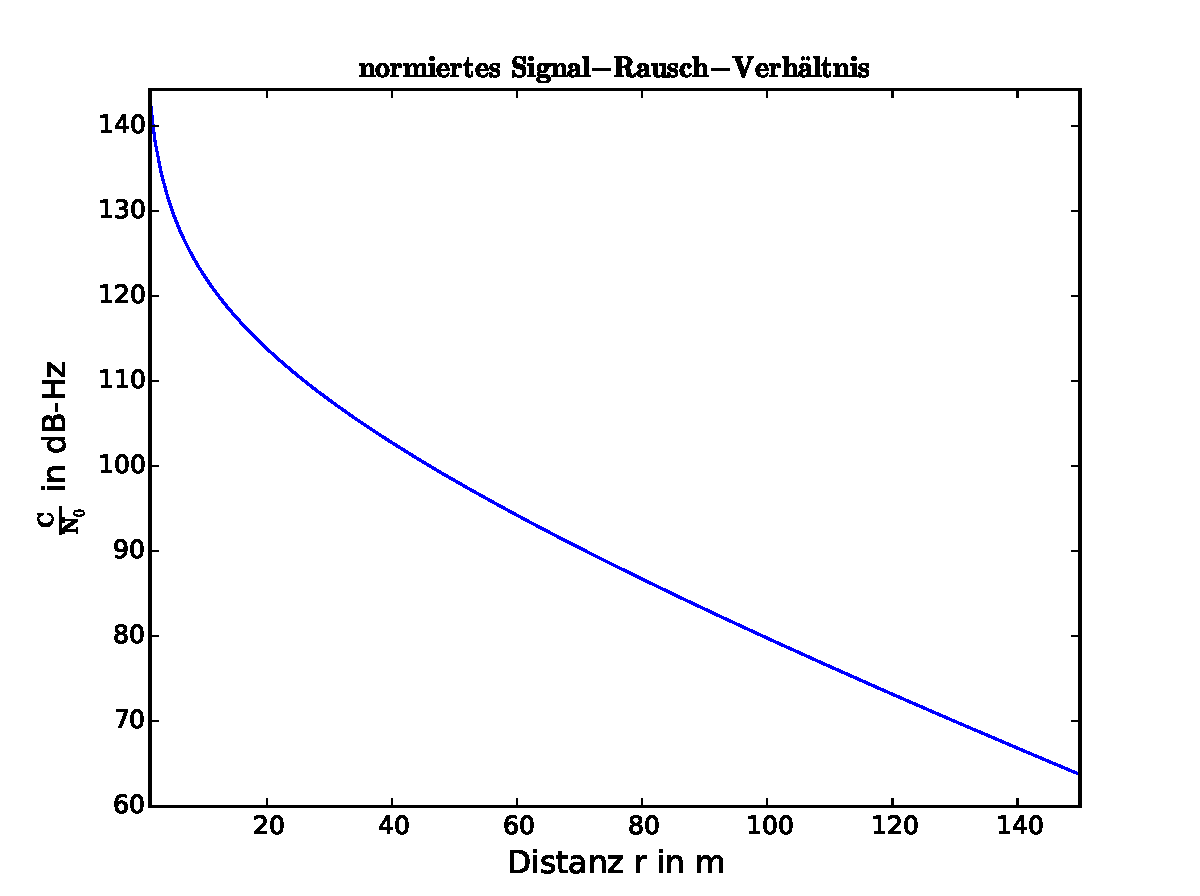
\includegraphics[width = 0.5\textwidth]{images/SNR_Distanz}} &
		\subfloat[\gls{CRLB}]{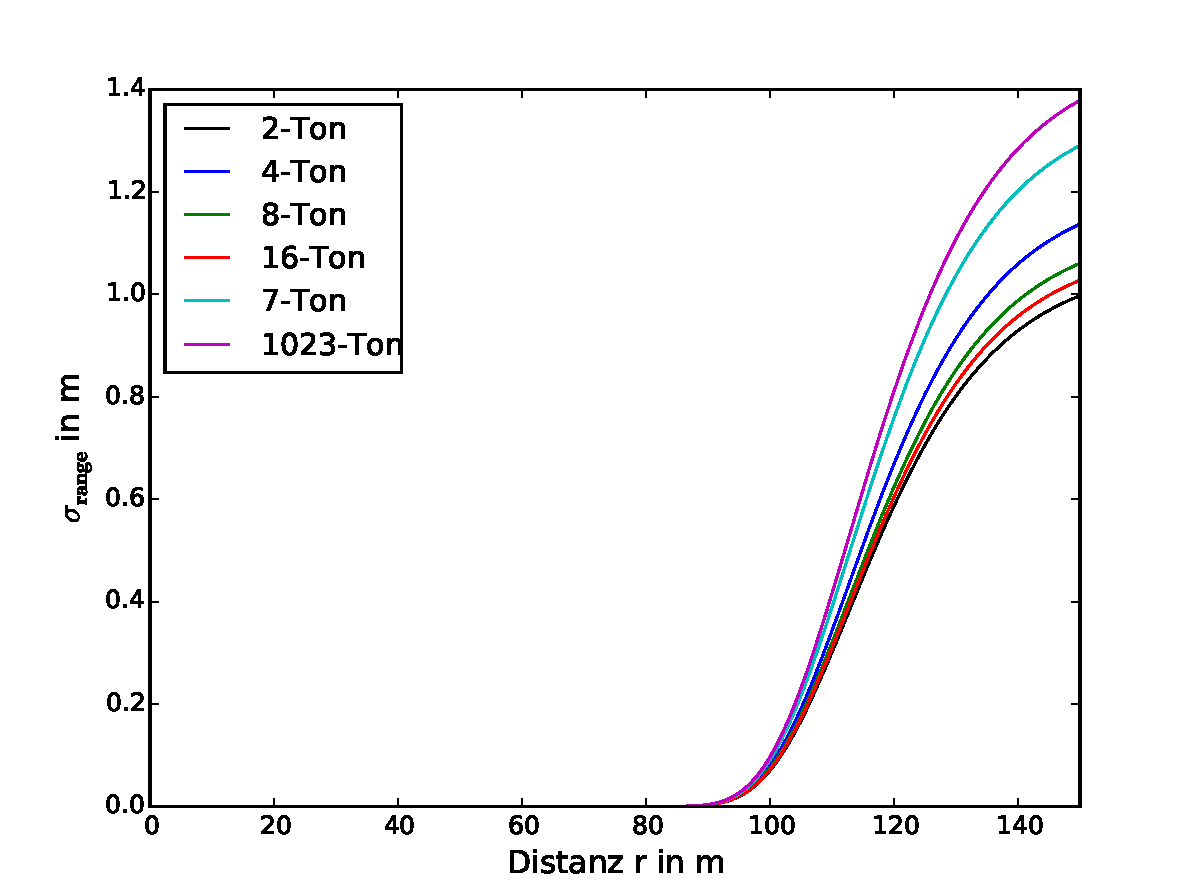
\includegraphics[width = 0.5\textwidth]{images/CRLB_Distanz}}	
	\end{tabular}}
	\caption{Distanzabhängige Auswirkung des \gls{AWGN}-Kanals auf das \nicefrac{\gls{symb:C}}{\gls{symb:N0}} und \gls{CRLB}}
	\label{fig:SNR_Distanz und CRLB}
\end{figure}

Mit kleiner werdenden \nicefrac[]{\gls{symb:C}}{\gls{symb:N0}}, wird die \gls{CRLB} nach \eqref{eq:CRLB_Range} größer. Aus diesem Grund weist sie ebenfalls eine Distanzabhängigkeit auf. Mit diesen Parametern ist es nun möglich die \gls{CRLB} nach \eqref{eq:CRLB_Range} für die Signale mit unterschiedlichem \gls{symb:brms} zu berechnen. Diese sind in \ref{fig:SNR_Distanz und CRLB}(b) abgebildet.
Der Abbildung \ref{fig:SNR_Distanz und CRLB}(a) ist des Weiteren zu entnehmen, dass bei einer Distanz von $\unit[150]{m}$ das \nicefrac[]{\gls{symb:C}}{\gls{symb:N0}}, Werte von $\unit[66]{dB-Hz}$ bis $\unit[140]{dB-Hz}$ annimmt. Anstatt die Auswertungen im Folgenden über die Distanz aufzutragen, werden sie über diesen Bereich des \nicefrac[]{\gls{symb:C}}{\gls{symb:N0}} veranschaulicht. In Abbildung \ref{fig:CRLB_SNR} ist die \gls{CRLB} der unterschiedlichen Signale im genannten Bereich des \nicefrac{\gls{symb:C}}{\gls{symb:N0}} abgebildet. Diese Kurven werden bei späteren Vergleichen als Referenz verwendet.
\begin{figure}[htbp]
	\centering
	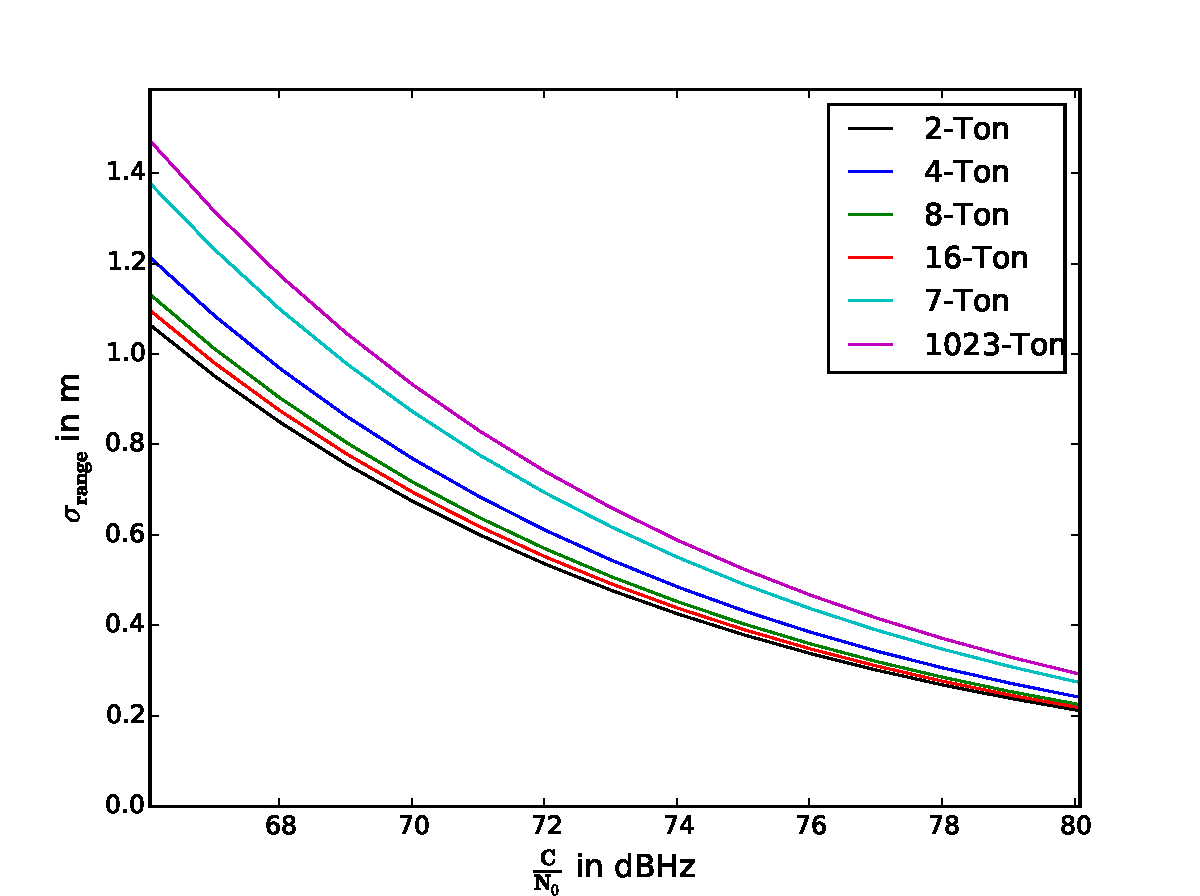
\includegraphics[width = 0.7\textwidth]{images/CRLB_Signale}
	\caption{\gls{CRLB} abhängig von \nicefrac[]{\gls{symb:C}}{\gls{symb:N0}}}
	\label{fig:CRLB_SNR}
\end{figure}
Lässt man alle anderen Parameter konstant, ist der 2-Ton das Signal mit der besten \gls{CRLB}. Ausgehend von diesem Signal sollte, bei weiterer Distribution der Energie, die Schranke größer werden. Dies wird in Abbildung \ref{fig:CRLB_SNR} bestätigt. Um wie viel sich die Schranke verschlechtert, ist von der Verteilung der Energie abhängig.
Je mehr Energie in Bandkantennähe ist, desto kleiner wird die Schranke. Die hier verwendeten Hadamard-Sequenzen haben die Eigenschaft, dass bei steigender Subträgerzahl, die stark gewichteten Subträger näher an die Bandkanten rücken. Damit liegt die Schranke des 16-Tons am nächsten an der des 2-Tons. 
Die $m$-Sequenzen sind nicht von diesem Effekt betroffen, da sie die Signalenergie immer auf alle Subträger gleich verteilen. Dadurch sind auch bei niedrigen Frequenzen, Subträger stark gewichtet, was folglich die \gls{CRLB} verschlechtert.


\subsection{Auswertung des gemittelten-Phasendifferenz-Schätzers}
\label{chap5.1.1:gemittelter Phasendifferenz Schätzer}
In diesem Abschnitt wird das Verhalten des gemittelten-Phasendifferenz-Schätzers, unter dem Einfluss des \gls{AWGN}-Kanals, untersucht. Es sollen Unterschiede, bei Verwendung der jeweiligen Testsignale, beobachtet und erläutert werden. 

\begin{figure}[htbp]
	\centering
	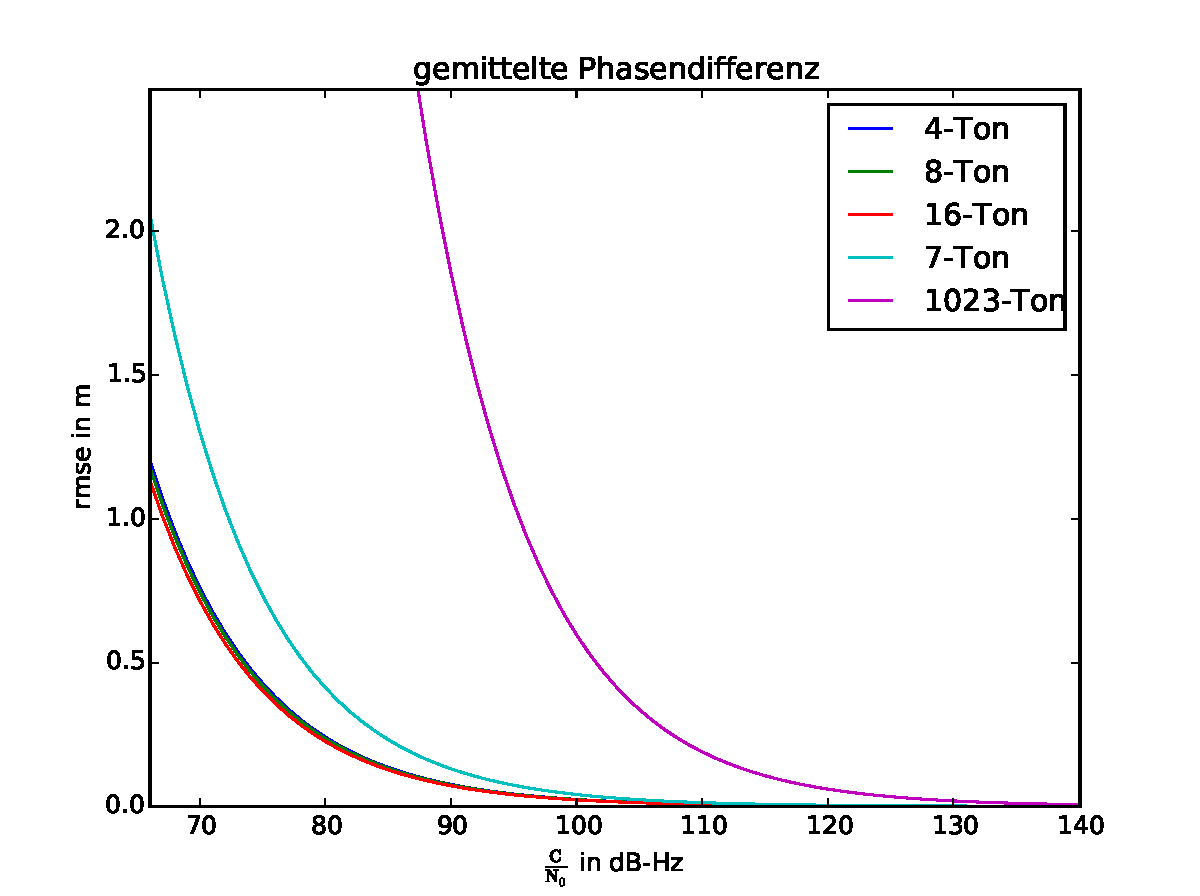
\includegraphics[width = 0.7\textwidth]{images/GemitteltePhasendiff_varianz}
	\caption{Simulation des Schätzfehlers der gemittelten Phasendifferenzschätzung bei einem \gls{AWGN}-Kanal}
	\label{fig:gemitteltePhasendiff_varianz}
\end{figure}

In Abbildung \ref{fig:gemitteltePhasendiff_varianz} ist zu sehen, dass die $m$-Sequenz mit 1023 Trägern stark von den restlichen Kurven abweicht. Grundsätzlich schneiden die $m$-Sequenzen im Vergleich zu den Hadamard-Sequenzen schlechter ab. Jedoch folgt dies, wie bereits erläutert, zwangsläufig aus der \gls{CRLB}.  
Um das Schätzverfahren unabhängig von der Signalcharakteristik zu evaluieren, wird der \gls{rmse} der einzelnen Signale mit der jeweiligen \gls{CRLB} aus Abbildung \ref{fig:CRLB_SNR} verglichen.

\begin{figure}[htbp]
	\centering
	\makebox[\textwidth][c]{\begin{tabular}{ccc}
			\subfloat[7-Ton]{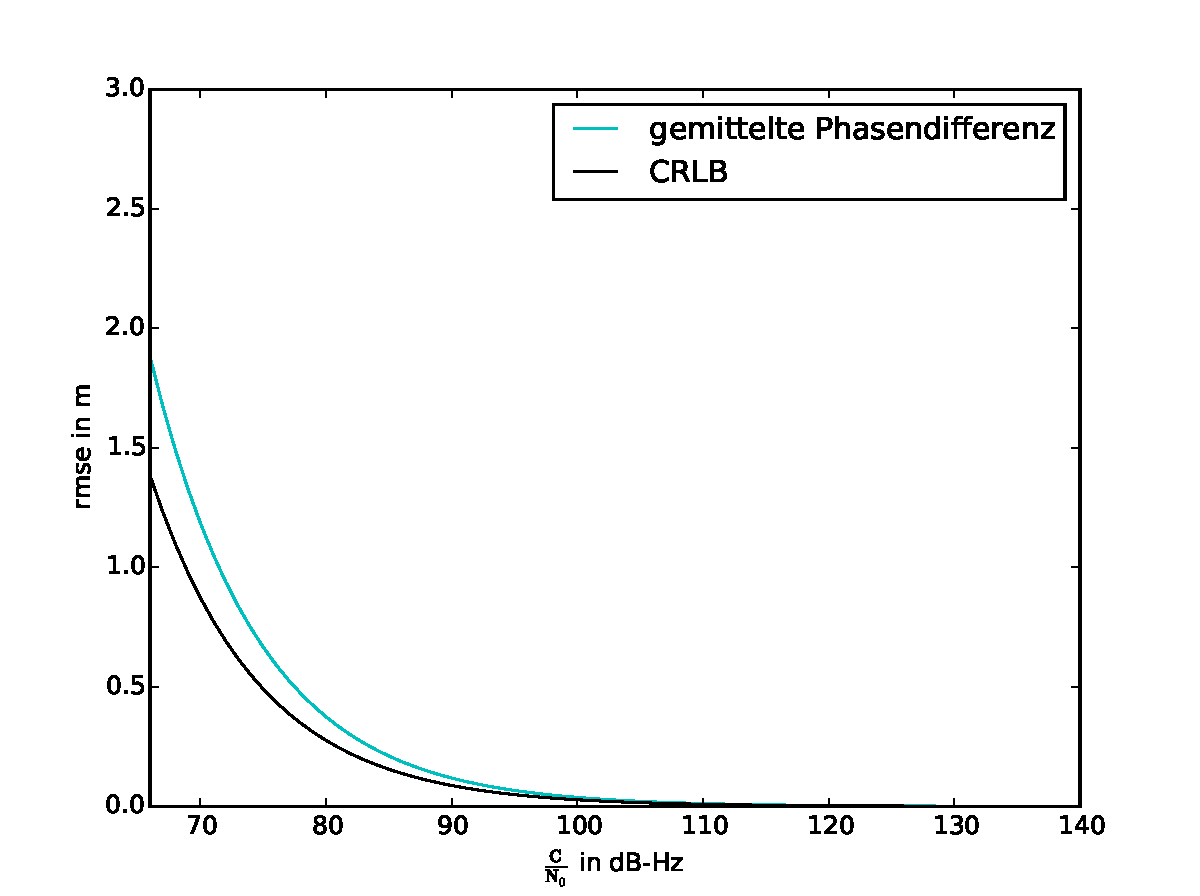
\includegraphics[width = 0.5\textwidth]{images/7-Ton_gegen_CRLB}} &
			\subfloat[1023-Ton]{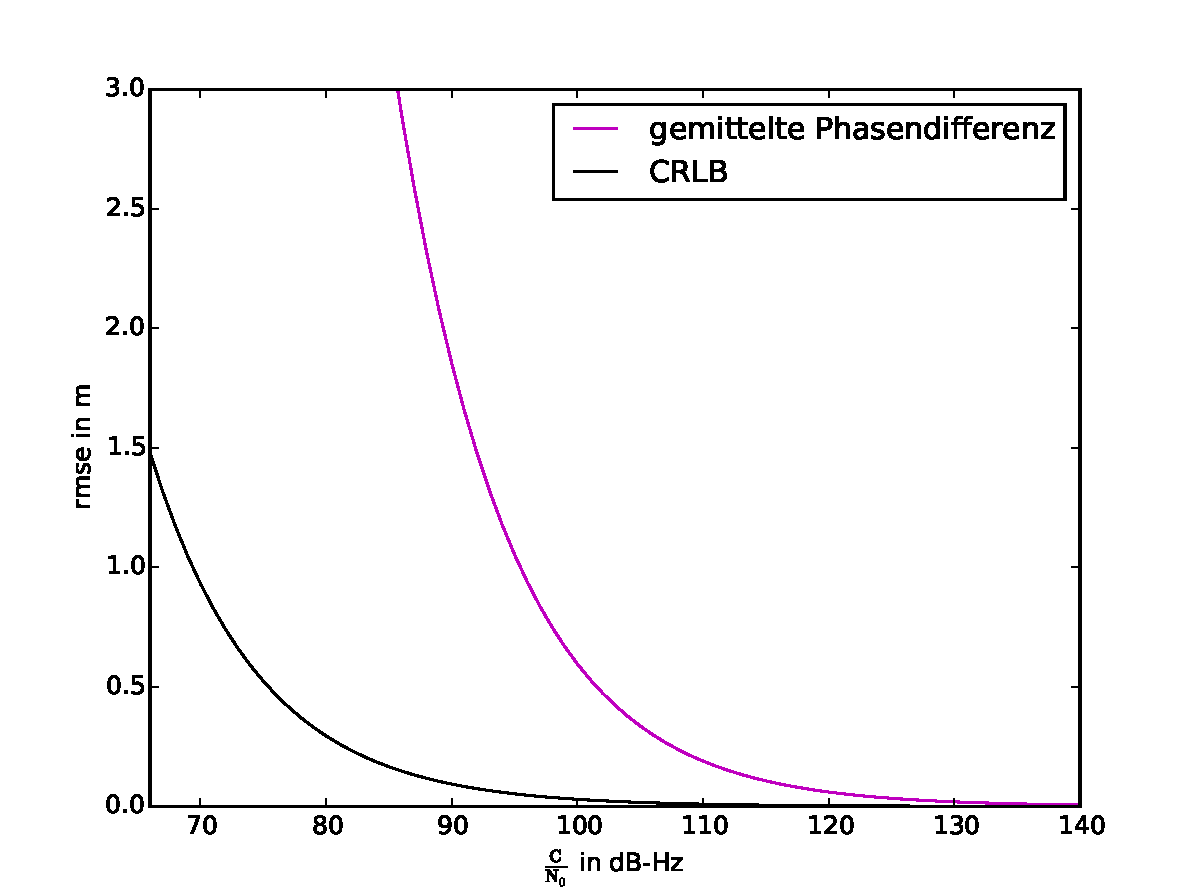
\includegraphics[width = 0.5\textwidth]{images/1023-Ton_gegen_CRLB}}
	\end{tabular}}
	\caption{\gls{rmse} der $m$-Sequenzen gegenüber der \gls{CRLB}}
	\label{fig:m_Phasendifferenz_CRLB_vergleich}
\end{figure}

Aus der Abbildung \ref{fig:m_Phasendifferenz_CRLB_vergleich} kann entnommen werden, dass dieses Schätzverfahren, bei Verwendung der $m$-Sequenzen, die untere Schranke nicht erreicht. Das ist bei den Hadamard-Sequenzen nicht der Fall.

\begin{figure}[htbp]
	\centering
	\makebox[\textwidth][c]{\begin{tabular}{ccc}	
		\subfloat[4-Ton]{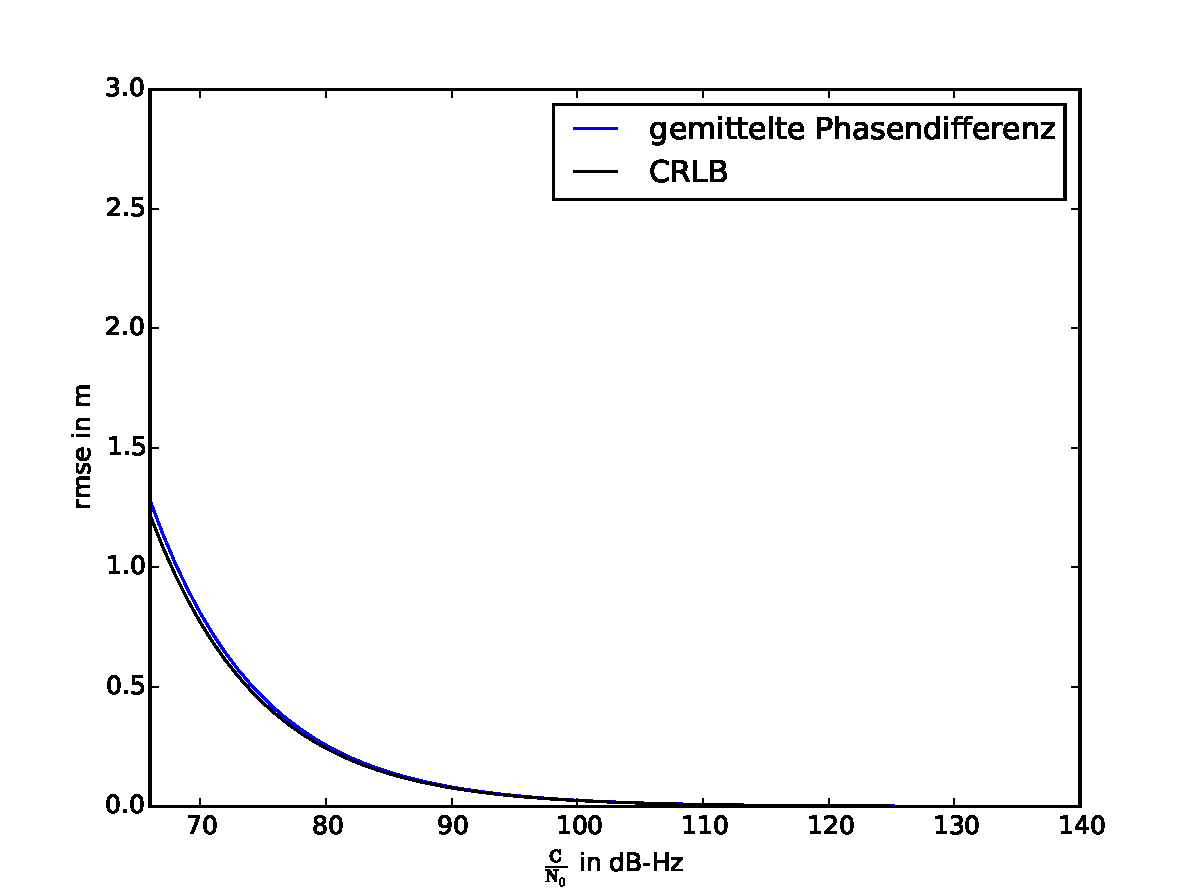
\includegraphics[width = 0.5\textwidth]{images/4-Ton_gegen_CRLB}}&
		\subfloat[8-Ton]{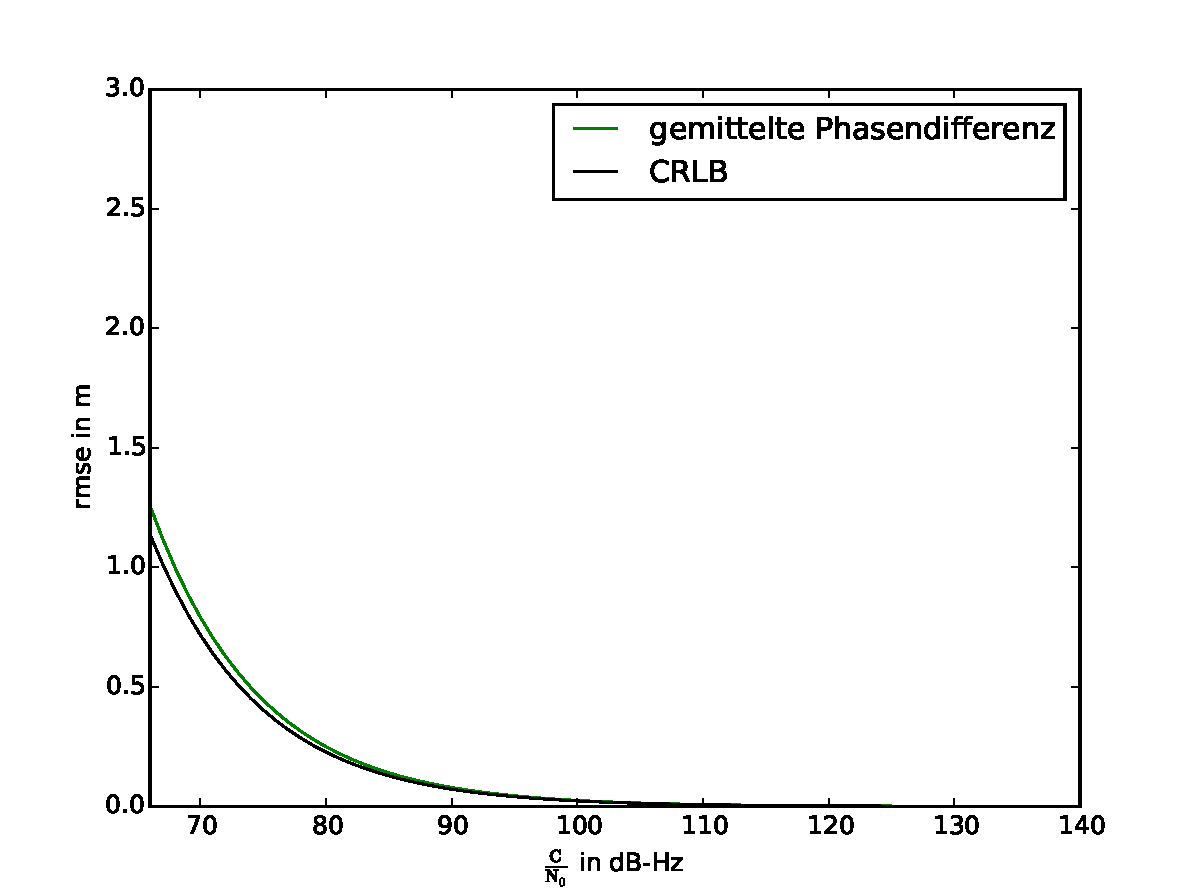
\includegraphics[width = 0.5\textwidth]{images/8-Ton_gegen_CRLB}}
		\end{tabular}}
	\makebox[\textwidth][c]{\begin{tabular}{ccc}
		\subfloat[16-Ton]{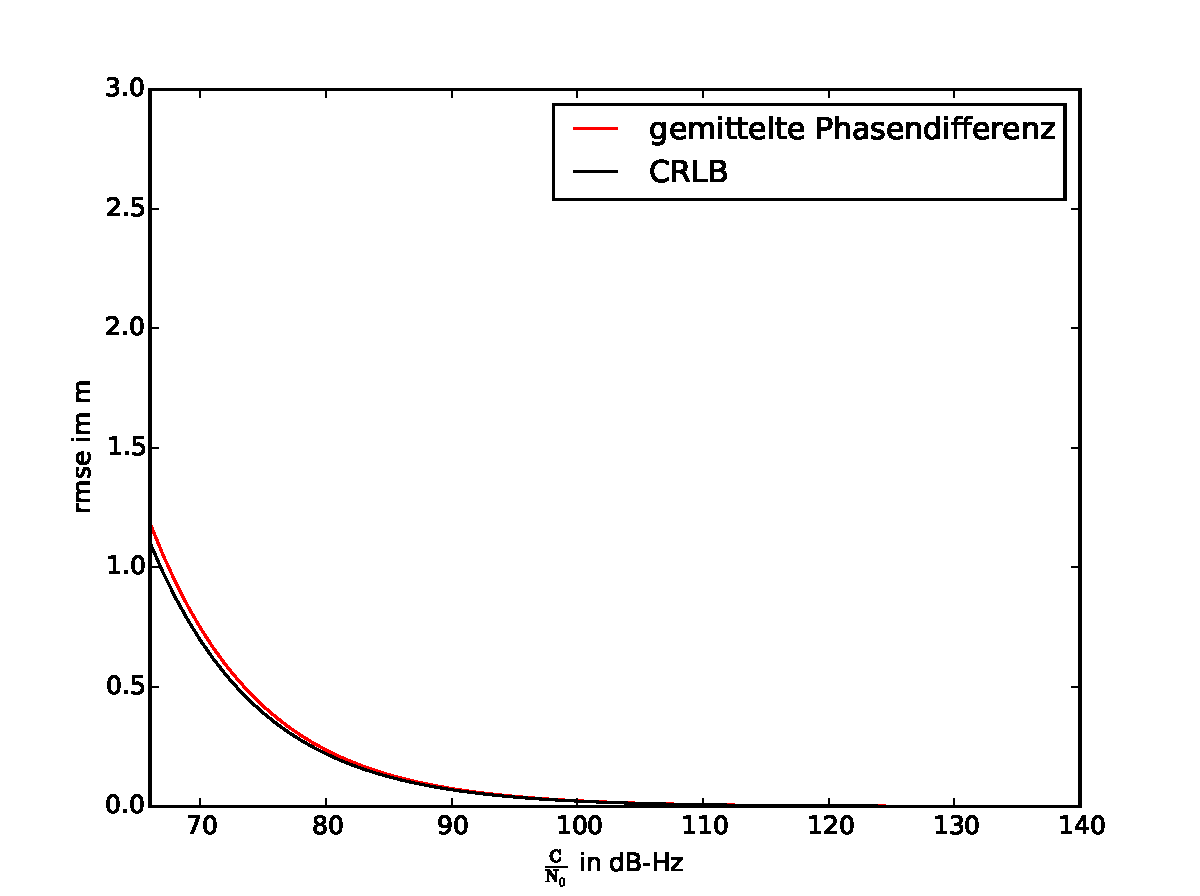
\includegraphics[width = 0.5\textwidth]{images/16-Ton_gegen_CRLB}}\\
	\end{tabular}}		
	\caption{\gls{rmse} der Hadamard-Sequenzen gegenüber der \gls{CRLB}}
	\label{fig:Had_Phasendifferenz_CRLB_vergleich}	
\end{figure}		
		
In Abbildung \ref{fig:Had_Phasendifferenz_CRLB_vergleich} ist zu sehen, dass für diese Signalformen dieser Schätzer die \gls{CRLB} nahezu für alle drei Testsignale erreicht. Welche Signalform am nächsten an der \gls{CRLB} liegt, kann aus Abbildung \ref{fig:m_Phasendifferenz_CRLB_vergleich} und \ref{fig:Had_Phasendifferenz_CRLB_vergleich} nicht klar abgelesen werden. Um eindeutig bestimmen zu können, welche Signalform die beste Leistung mit den hier verwendeten Schätzverfahren erzielt, muss die Schätzeffizienz nach \eqref{eq:e} betrachtet werden. Sie nimmt Werte zwischen 0 und 1 an, wobei die maximale Schätzeffizienz erreicht ist, wenn die Varianz des Schätzfehlers auf der \gls{CRLB} liegt. 

\begin{figure}[htbp]
	\centering
	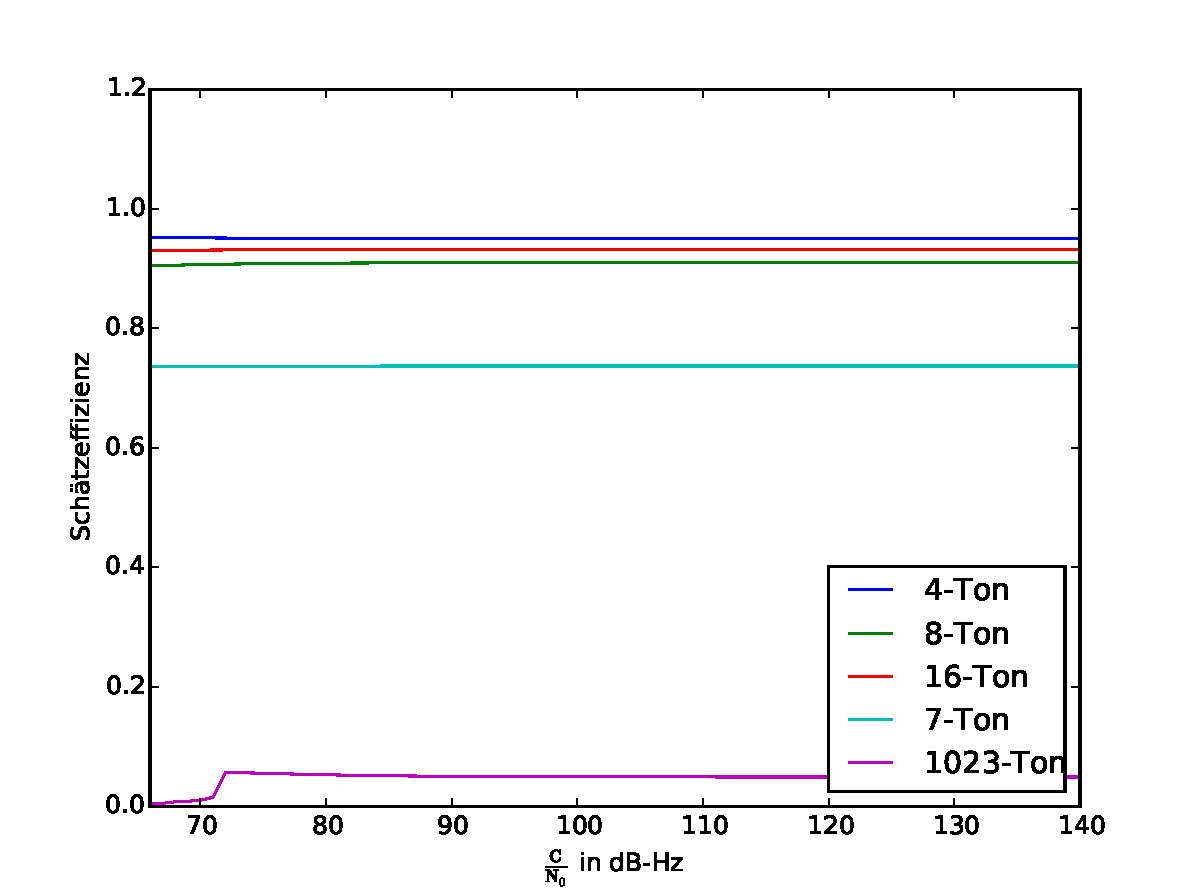
\includegraphics[width = 0.7\textwidth]{images/Schaetzeffizienz}
	\caption{Schätzeffizienz des gemittelten Phasendifferenz-Schätzers}
	\label{fig:Schätzeffizienz}
\end{figure} 

Durch Abbildung \ref{fig:Schätzeffizienz} wird ersichtlich, dass die höchste Schätzeffizienz mit dem 4-Ton erreicht wird. Zumal jedoch das Schätzverfahren beim 16-Ton eine höhere Effizienz als beim 8-Ton aufweist, kann eine steigende Subträgerzahl nicht mit einer zunehmenden Schätzeffizienz verknüpft werden. Welche Effizienz das Schätzverfahren mit einem Signal erreicht hängt lediglich von den Positionen der Subträger bzw. der Energieverteilung im Band ab.  

\subsection{Auswertung des L\texorpdfstring{$\&$}{TEXT}R-Schätzers}
\label{chap5.1.2:LundR Auswertung}
In Abbildung \ref{fig:LundR_varianz} ist der \gls{rmse} des L$\&$R-Schätzers unter Verwendung der fünf Testsignale aufgetragen. 

\begin{figure}[htbp]
	\centering
	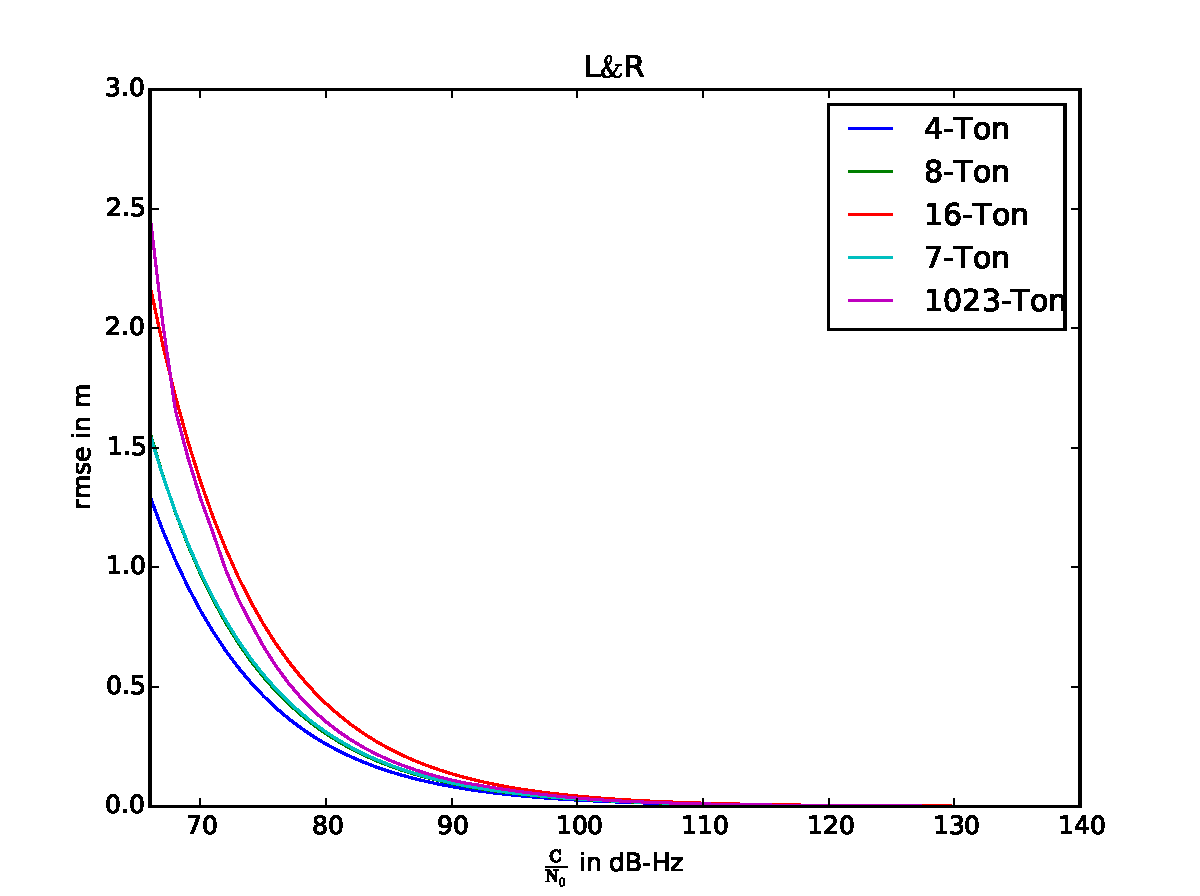
\includegraphics[width = 0.7\textwidth]{images/LundR_varianz}
	\caption{Simulation des Schätzfehlers des L$\&$R-Schätzers bei einem \gls{AWGN}-Kanal}
	\label{fig:LundR_varianz}
\end{figure}

Darin ist zu sehen, dass die $m$-Sequenzen weniger große Fehler, als beim gemittelten-Phasendifferenz-Schätzer verursachen. Um eine genauere Aussage über die Leistungsfähigkeit des L$\&$R-Schätzers zu treffen soll zunächst der Vergleich mit der \gls{CRLB} in den Abbildungen \ref{fig:Had_LuR_CRLB_vergleich} und \ref{fig:m_LuR_CRLB_vergleich} betrachtet werden. 
Die Hadamard-Sequenzen sorgen bei diesem Schätzverfahren, mit steigender Subträgerzahl, für einen größer werdenden Fehler. Die Fehlerkurven der $m$-Sequenzen kommen jedoch an die \gls{CRLB} heran.

\begin{figure}[htbp]
	\centering
	\makebox[\textwidth][c]{\begin{tabular}{cccc}
		\subfloat[4-Ton]{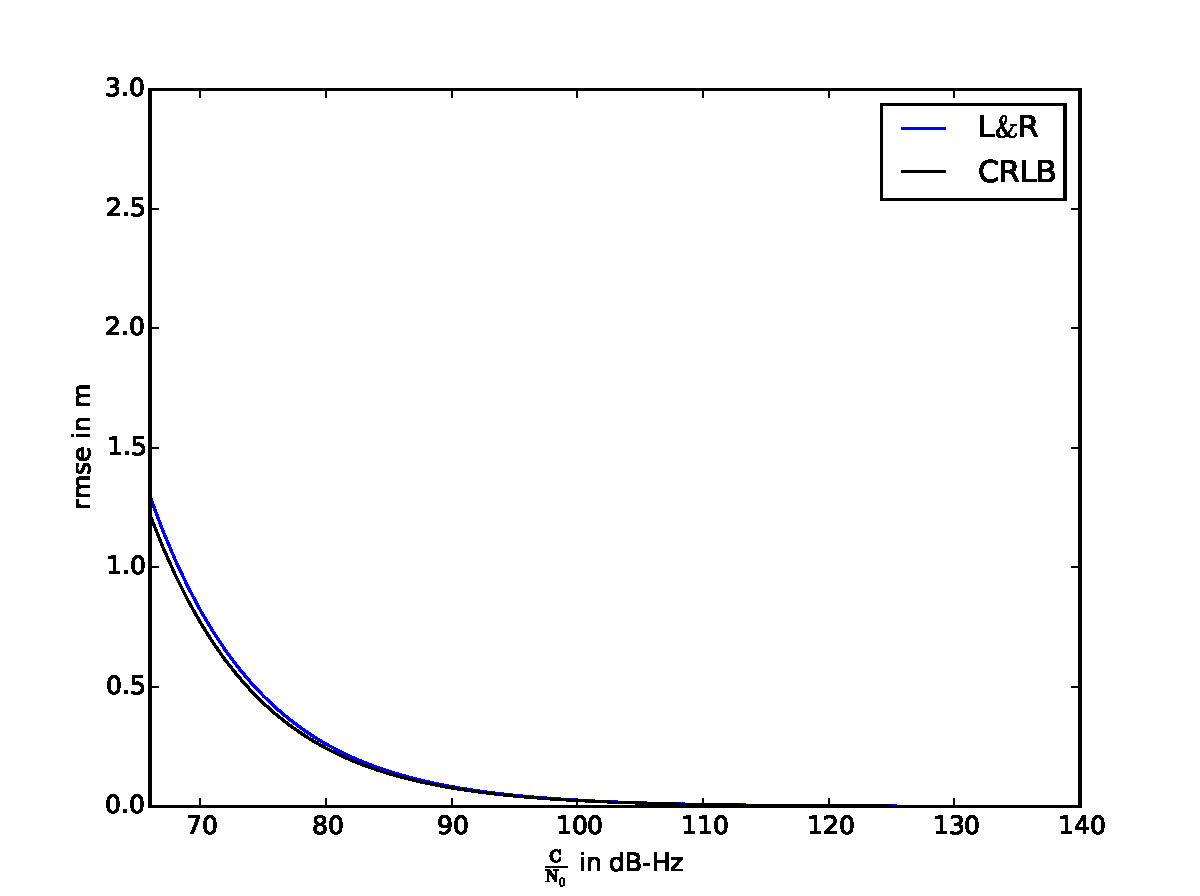
\includegraphics[width=0.5\textwidth]{images/LR4-Ton_gegen_CRLB}} &
		\subfloat[8-Ton]{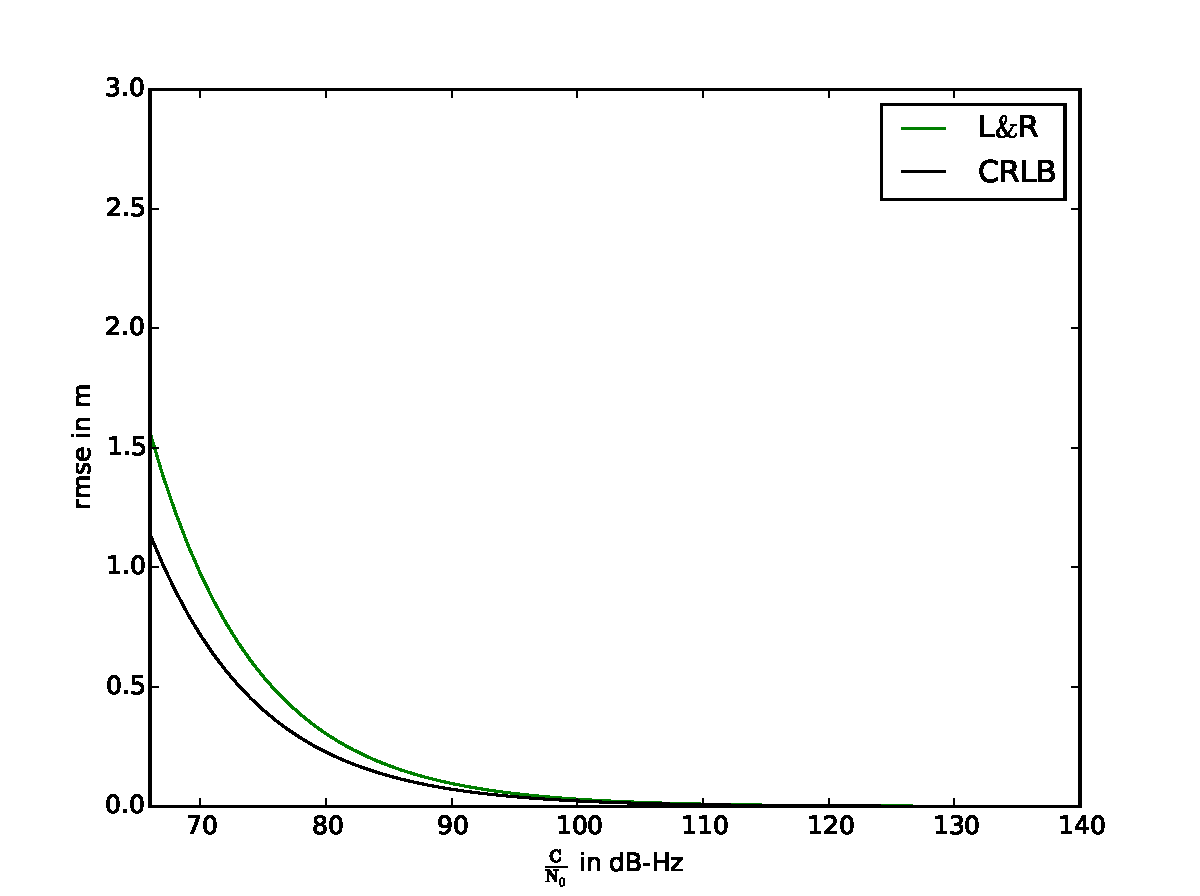
\includegraphics[width=0.5\textwidth]{images/LR8-Ton_gegen_CRLB}}
	\end{tabular}}
		
	\makebox[\textwidth][c]{\begin{tabular}{cccc}
		\subfloat[16-Ton]{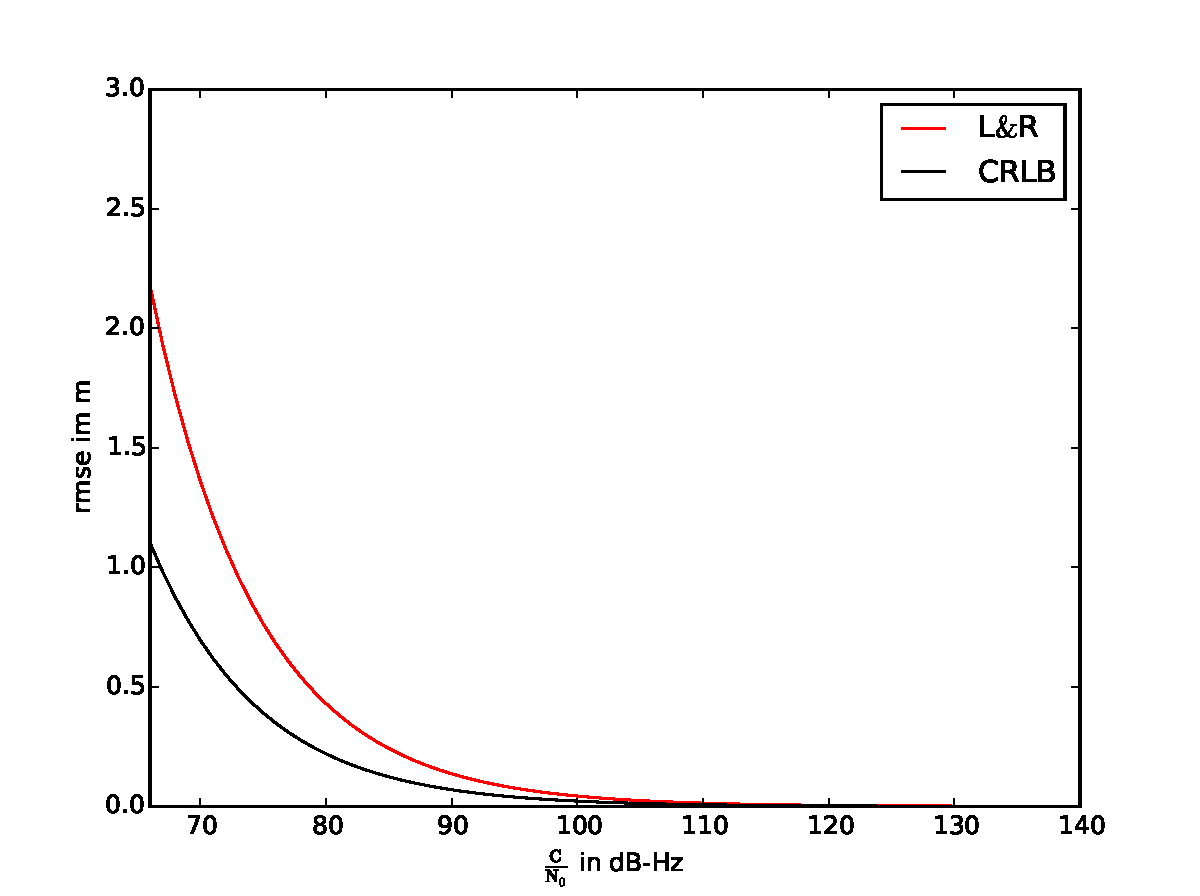
\includegraphics[width=0.5\textwidth]{images/LR16-Ton_gegen_CRLB}}
	\end{tabular}}
	
	\caption{\gls{rmse} des L$\&$R-Schätzers mit Hadamard-Sequenzen gegenüber der \gls{CRLB}}
	\label{fig:Had_LuR_CRLB_vergleich}	
\end{figure}

Eine Erklärungsmöglichkeit für die schlechten Ergebnisse der Hadamard-Sequenzen, kann in der Gleichung \eqref{eq:Approximation} gefunden werden. Darin wird eine Vereinfachung für eine Summe von Exponentialfunktionen vorgenommen. Der Ansatz geht jedoch davon aus, dass alle $e$-Funktionen gleich gewichtet sind. Da die Subträger der Hadamard-Sequenzen unterschiedliche Gewichte haben, trifft diese Vereinfachung nicht auf diese Signalform zu. Bei zunehmender Subträgerzahl werden diese Abweichungen immer größer. Um das Schätzverfahren trotzdem auswerten zu können, wurden die Subträger der Signale nachträglich skaliert, damit sie die selben Gewichte haben. Diese Maßnahme verschlechtert jedoch das \nicefrac[]{\gls{symb:C}}{\gls{symb:N0}}, da das Rauschen ebenfalls skaliert wird. Diese Fehlerquelle zeigt, dass der \gls{LuR}-Schätzer suboptimal für diese Art von Signalen ist. Um den \gls{rmse} an die \gls{CRLB} anzunähern, müsste die Approximation \eqref{eq:Approximation} nochmals für unterschiedlich gewichtete e-Funktionen hergeleitet werden. Dies überschreitet jedoch den Umfang dieser Arbeit, da nicht einmal erwiesen ist, ob eine solche Vereinfachung für unterschiedlich gewichtete Exponentialfunktionen überhaupt existiert. 

\begin{figure}[htbp]
	\centering
	\makebox[\textwidth][c]{\begin{tabular}{ccc}
		\subfloat[7-Ton]{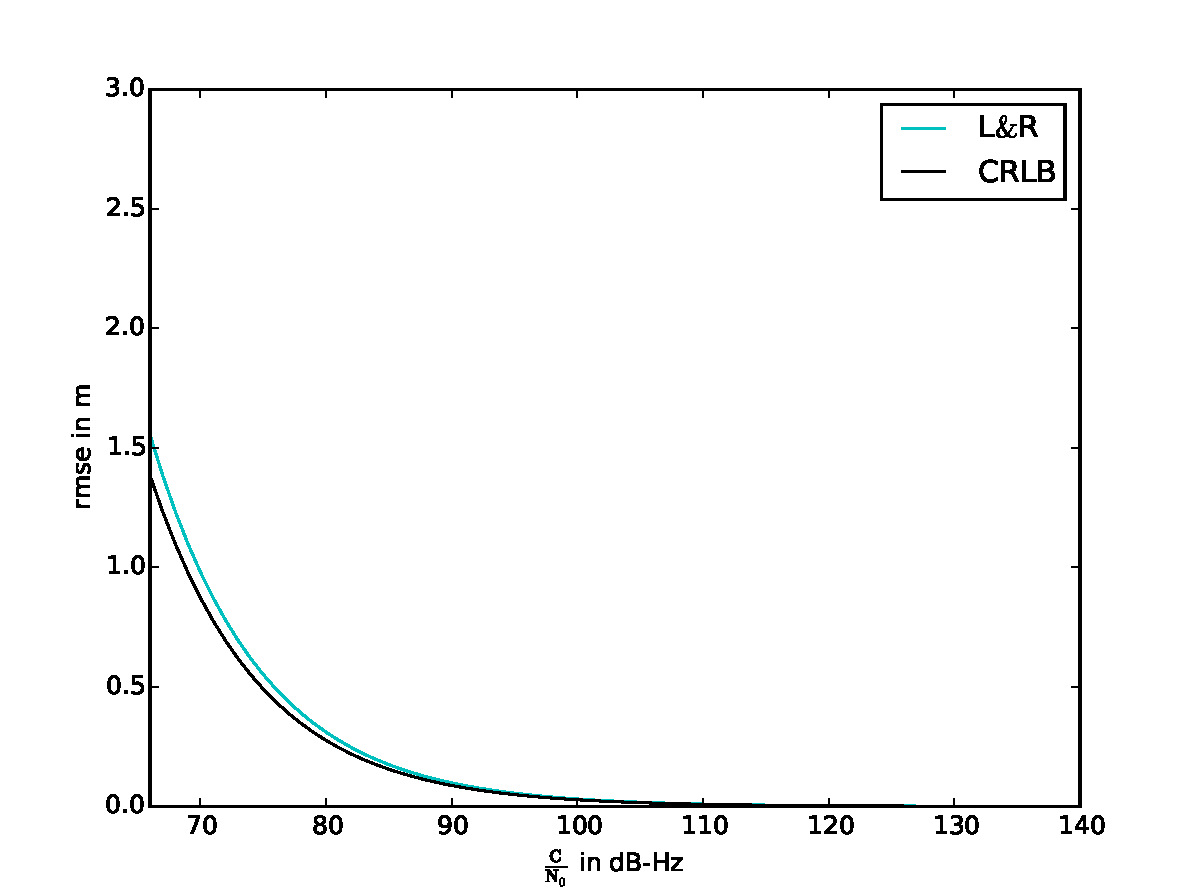
\includegraphics[width=0.5\textwidth]{images/LR7-Ton_gegen_CRLB}} &
		\subfloat[1024-Ton]{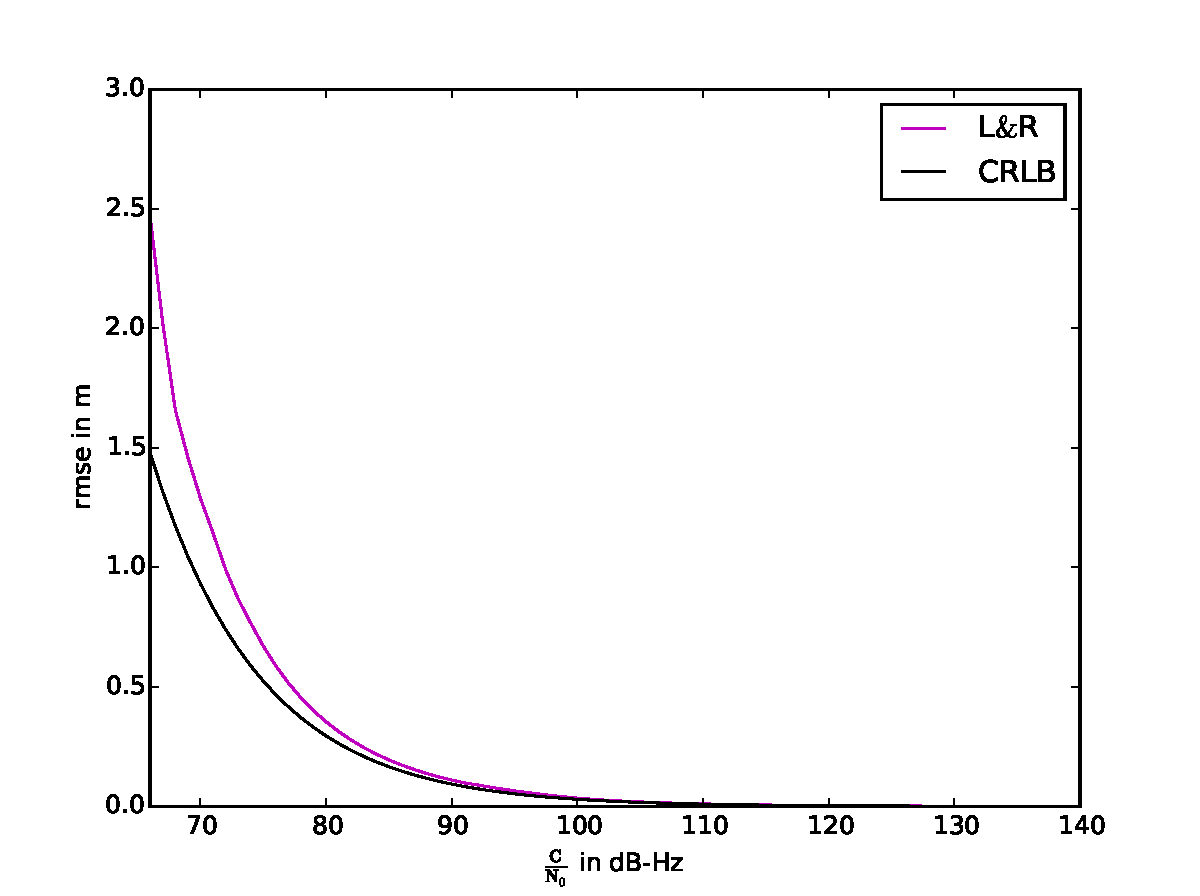
\includegraphics[width=0.5\textwidth]{images/LR1023-Ton_gegen_CRLB}}
	\end{tabular}}
	\caption{\gls{rmse} des L$\&$R-Schätzers mit $m$-Sequenzen gegenüber der \gls{CRLB}}
	\label{fig:m_LuR_CRLB_vergleich}
\end{figure}

Die $m$-Sequenzen erfüllen die Bedingung zwar bei ihrer Erzeugung, sind jedoch nach der Impulsformung mit einer Sinc-Funktion im Frequenzbereich gewichtet. Daher gilt diese Vereinfachung für sie ebenfalls nicht. Der Fehler scheint allerdings bei ihnen nicht so stark ins Gewicht zu fallen. Laut \cite[S.90]{mengali1997synchronization} ist die wesentliche Verbesserung dieses Schätzverfahrens gegenüber anderen Mittelungsverfahren, dass das \nicefrac[]{\gls{symb:C}}{\gls{symb:N0}}, durch die zusätzliche Glättung des Rauschens in Gleichung \eqref{eq:rauschglaettung} verbessert wird. Dies könnte eine Begründung dafür sein, wieso sich die $m$-Sequenzen im Vergleich zum gemittelten-Phasendifferenz-Schätzers, so stark verbessern, obwohl sie ungleiche Subträgergewichte aufweisen. Zum einen ist der Unterschied der Subträgergewichte nach der Impulsformung nicht so groß wie bei den Hadamard-Sequenzen und zum anderen besitzen sie mehr Phasenwerte, über welche gemittelt werden kann. 
An der Schätzeffizienz in Abbildung \ref{fig:LuRSChätzeffizienz} ist zu sehen wie stark die $m$-Sequenzen sich verbessern. Bei dem 7-Ton ist die Verbesserung nur noch minimal, da diese Signalform beim gemittelten Phasendifferenz-Schätzer schon einen Verlauf ähnlich der \gls{CRLB} hatte.
Aus der Schätzeffizienz aller Signale kann wiederum bestimmt werden, welche die geeignetste Signalform für diesen Schätzer ist. 
\begin{figure}[htbp]
	\centering
	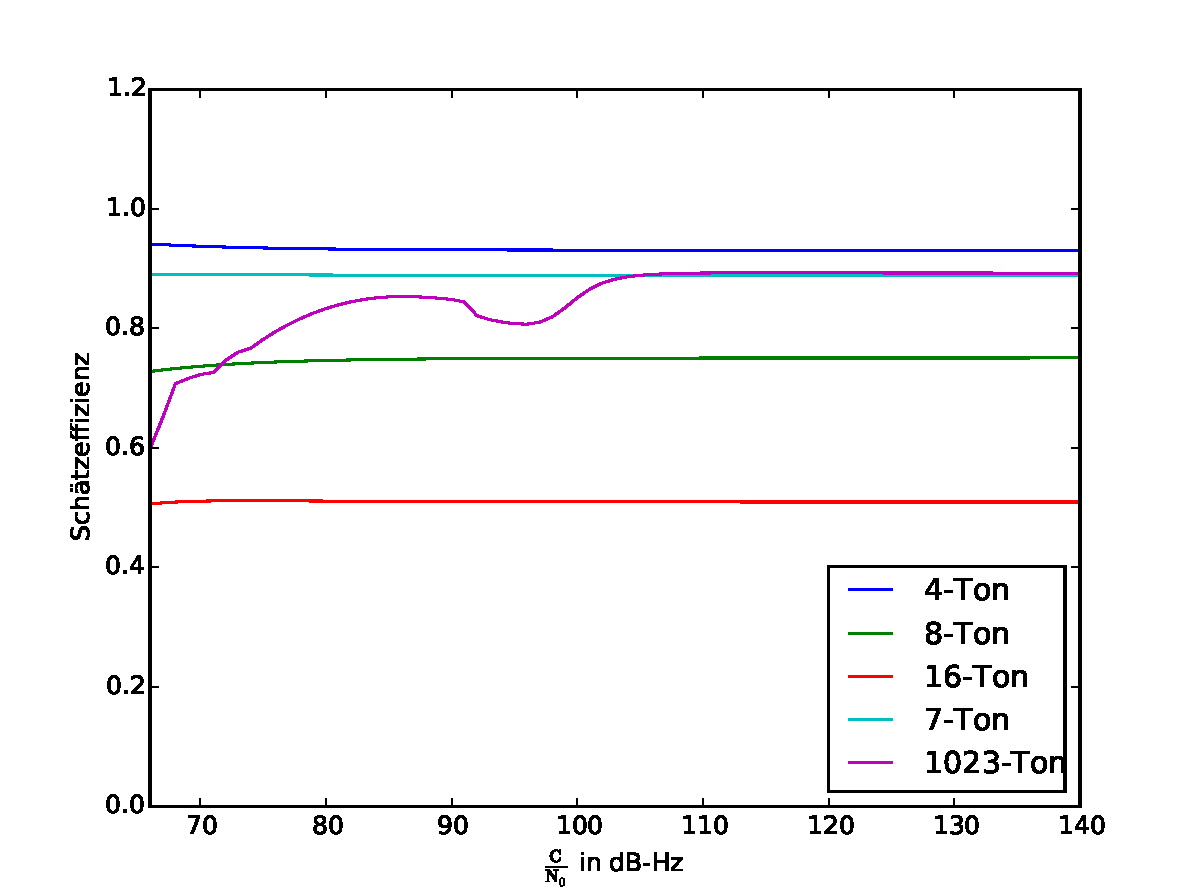
\includegraphics[width = 0.7\textwidth]{images/LuRschaetzeffizienz}
	\caption{Schätzeffizienz des L$\&$R-Schätzers}
	\label{fig:LuRSChätzeffizienz} 
\end{figure}
Die Effizienz des 1023-Ton ist für ein gutes \nicefrac[]{\gls{symb:C}}{\gls{symb:N0}} sehr hoch, fällt jedoch bei kleiner werdenden \nicefrac[]{\gls{symb:C}}{\gls{symb:N0}} stark ab. Der 7-Ton und 4-Ton weisen die höchste Effizienz bei diesen Schätzverfahren auf. Im Vergleich zu ihnen, sind die Signale des 8- und 16-Tons äußerst ineffizient.

\subsection{Auswertung von MUSIC und ESPRIT}
\gls{MUSIC} und \gls{ESPRIT} arbeiten im selben Subraum und haben deshalb ähnliche Ergebnisse in der Auswertung. Lediglich die Art und Weise, wie die Laufzeitinformation aus dem Subraum extrahiert wird, unterscheidet sich bei diesen Verfahren.

\begin{figure}[htbp]
	\centering
	\makebox[\textwidth][c]{\begin{tabular}{ccc}
		\subfloat[\gls{MUSIC}]{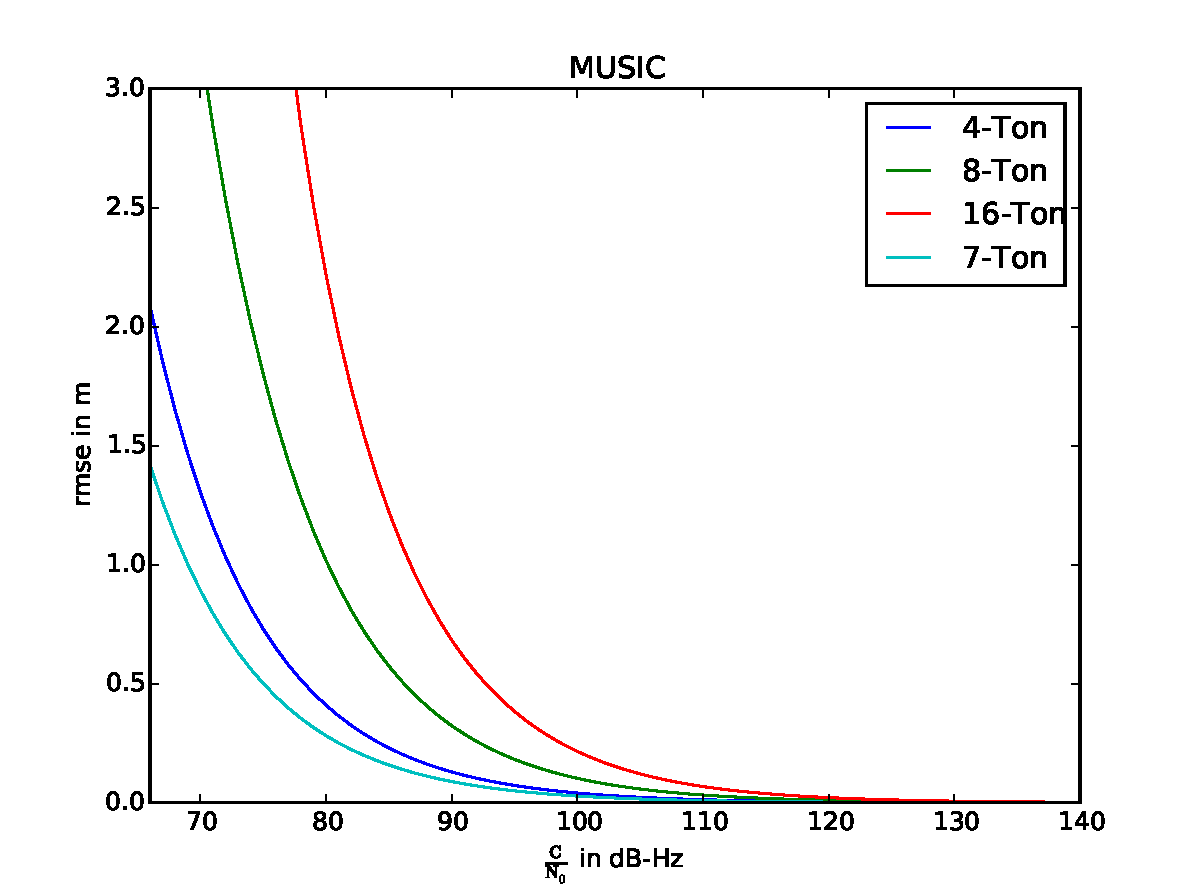
\includegraphics[width = 0.5\textwidth]{images/MUSIC_varianz}} &
		\subfloat[\gls{ESPRIT}]{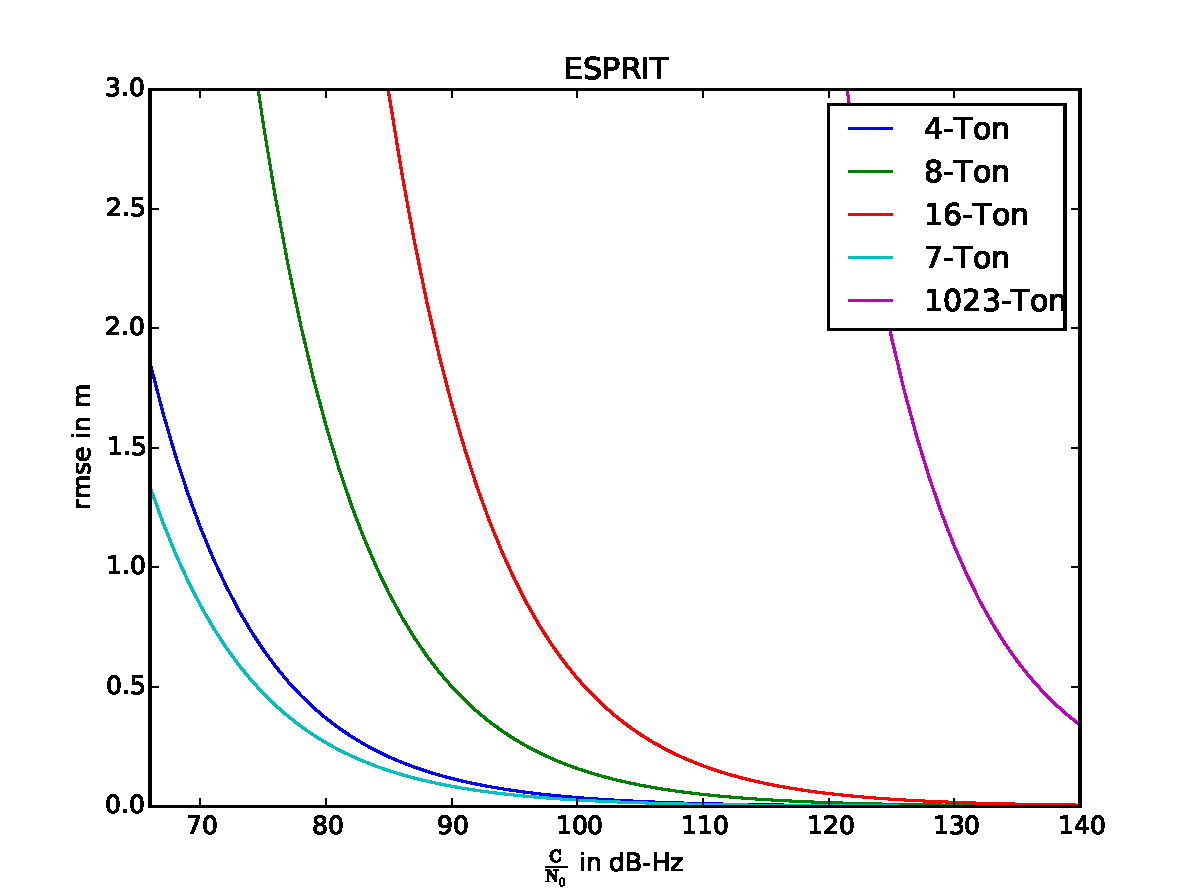
\includegraphics[width = 0.5\textwidth]{images/ESPRIT_varianz}}
	\end{tabular}}
	\caption{Simulation des Schätzfehlers des \gls{ESPRIT}- und \gls{MUSIC}-Schätzers bei einem \gls{AWGN}-Kanal}
	\label{fig:ESPRIT_MUSIC_varianz}
\end{figure}

In Abbildung \ref{fig:ESPRIT_MUSIC_varianz} ist zu sehen, dass die Kurven ähnliche Verläufe aufzeigen. Eine Auswertung für den 1023-Ton  war mit dem Root-\gls{MUSIC} Algorithmus jedoch nicht möglich, da dieser mit der hohen Anzahl an Subträgern einen zu hohen Rechenaufwand benötigt. 
Die Fehlerkurven aller Signale steigen bei kleinen \nicefrac[]{\gls{symb:C}}{\gls{symb:N0}} stark an. Zunächst wird \gls{ESPRIT} ausgewertet.
Lediglich der 7-Ton bleibt in der Nähe der \gls{CRLB}, wie in den Abbildungen \ref{fig:Had_ESPRIT_CRLB_vergleich} und \ref{fig:m_ESPRIT_CRLB_vergleich} zu sehen ist. 

\begin{figure}[htbp]
	\centering
	\makebox[\textwidth][c]{
	\begin{tabular}{cccc}	
		\subfloat[4-Ton]{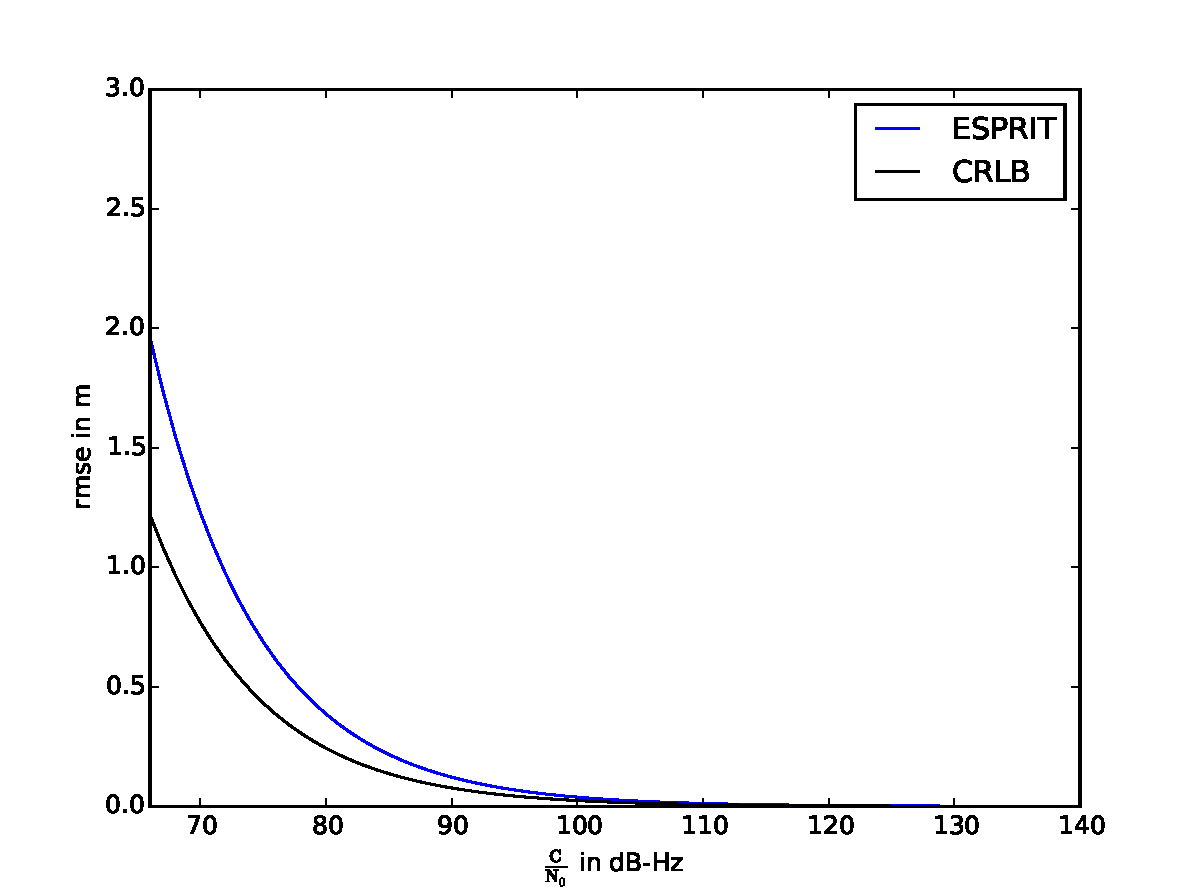
\includegraphics[width = 0.5\textwidth]{images/ESPRIT_4Ton_CRLB}} &
		\subfloat[8-Ton]{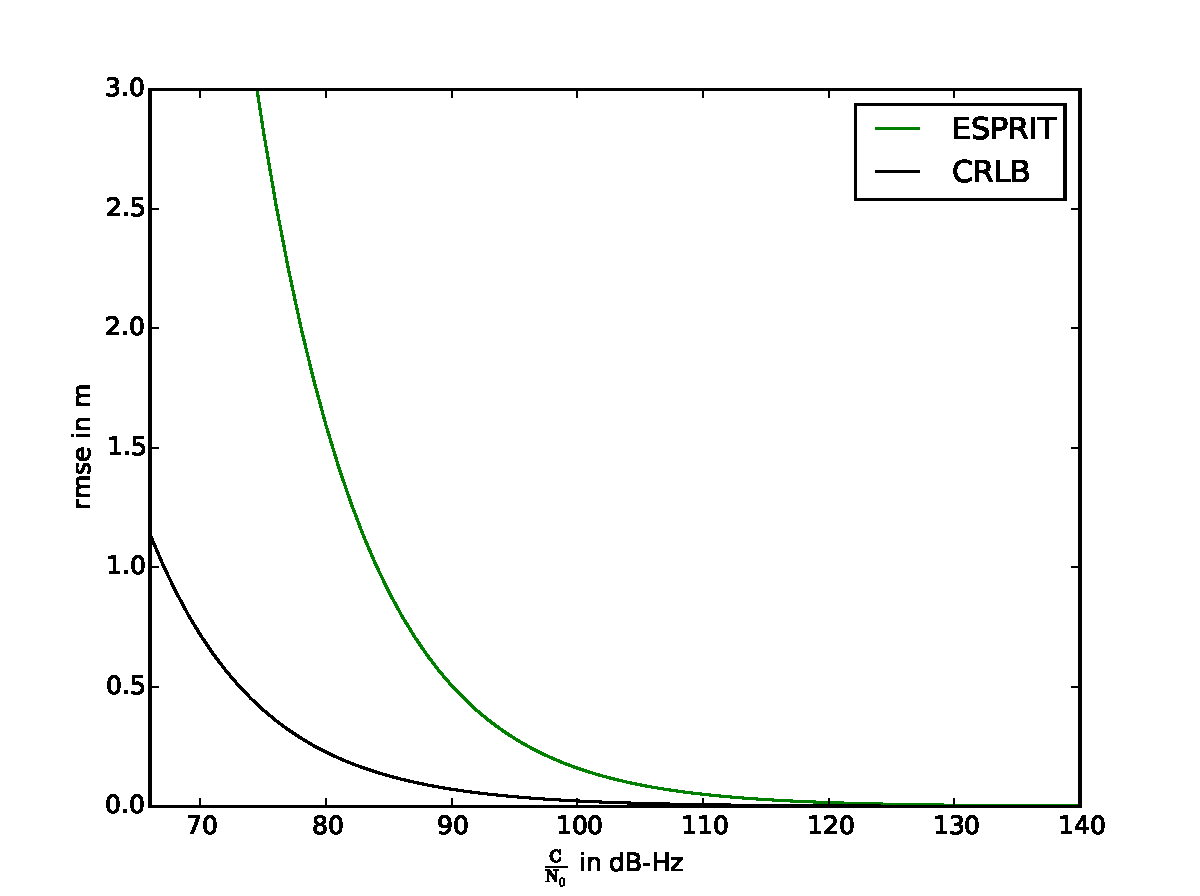
\includegraphics[width = 0.5\textwidth]{images/ESPRIT_8Ton_CRLB}}
		\end{tabular}}	
		
	\makebox[\textwidth][c]{\begin{tabular}{ccc}
		\subfloat[16-Ton]{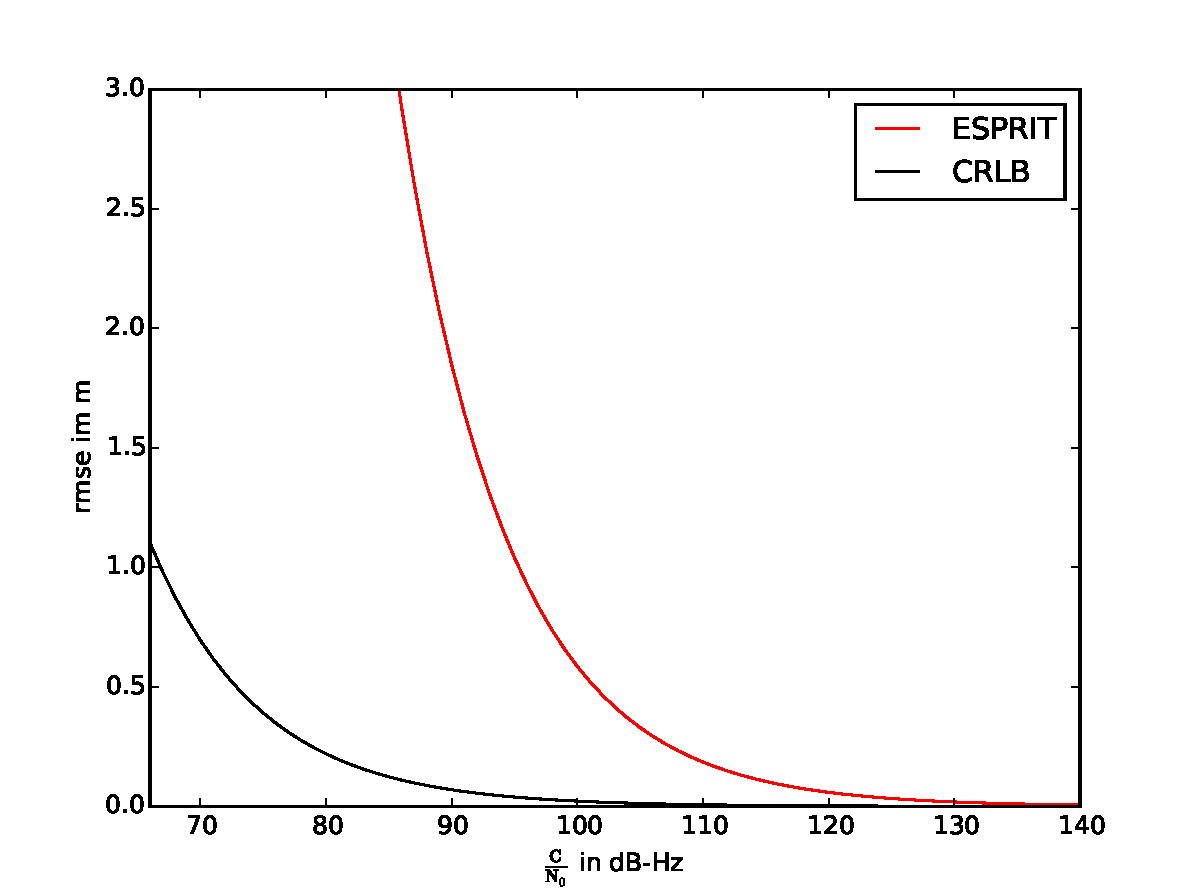
\includegraphics[width = 0.5\textwidth]{images/ESPRIT_16Ton_CRLB}}
			\end{tabular}}
	\caption{Varianz des \gls{ESPRIT}-Schätzers gegenüber der \gls{CRLB} für Hadamard-Sequnzen}
	\label{fig:Had_ESPRIT_CRLB_vergleich}
\end{figure}

Auffällig ist, dass die Hadamard-Sequenzen besonders stark von der \gls{CRLB} abweichen.
Bei genauerer Betrachtung des Schätzablaufes, wird ersichtlich, dass ein Fehler bei der Kanalschätzung, nach \eqref{eq:Übertragungsfunktion}, gemacht wird, wenn die Subträger nicht gleich gewichtet sind. Es handelt sich wieder um ein ähnliches Problem, wie beim \gls{LuR}-Schätzer. Wenn die Subträger nicht gleich gewichtet sind, wird bei der Bildung des Quotienten, jeder Subträger mit sich selbst normiert. Dadurch werden Subträger skaliert und verschlechtern somit das \nicefrac[]{\gls{symb:C}}{\gls{symb:N0}}. Als Lösung dieses Problems, würde sich anbieten anstelle der Quotientenbildung ein komplex konjugiertes Produkt des Empfangsspektrums $R(f)$ und des Sendespektrums $S(f)$ zu berechnen. Damit gehen jedoch erhebliche Veränderungen an den Algorithmen einher.  Anstrengungen dieses Problem zu umgehen, führten allerdings zu keiner Verbesserung des Schätzfehlers. Somit zeigt der \gls{rmse} dieses Schätzers, dass die Algorithmen Signale mit gleich gewichteten Subträgern benötigen. 

\begin{figure}[htbp]
	\centering
	\makebox[\textwidth][c]{	
	\begin{tabular}{cccc}
		\subfloat[7-Ton]{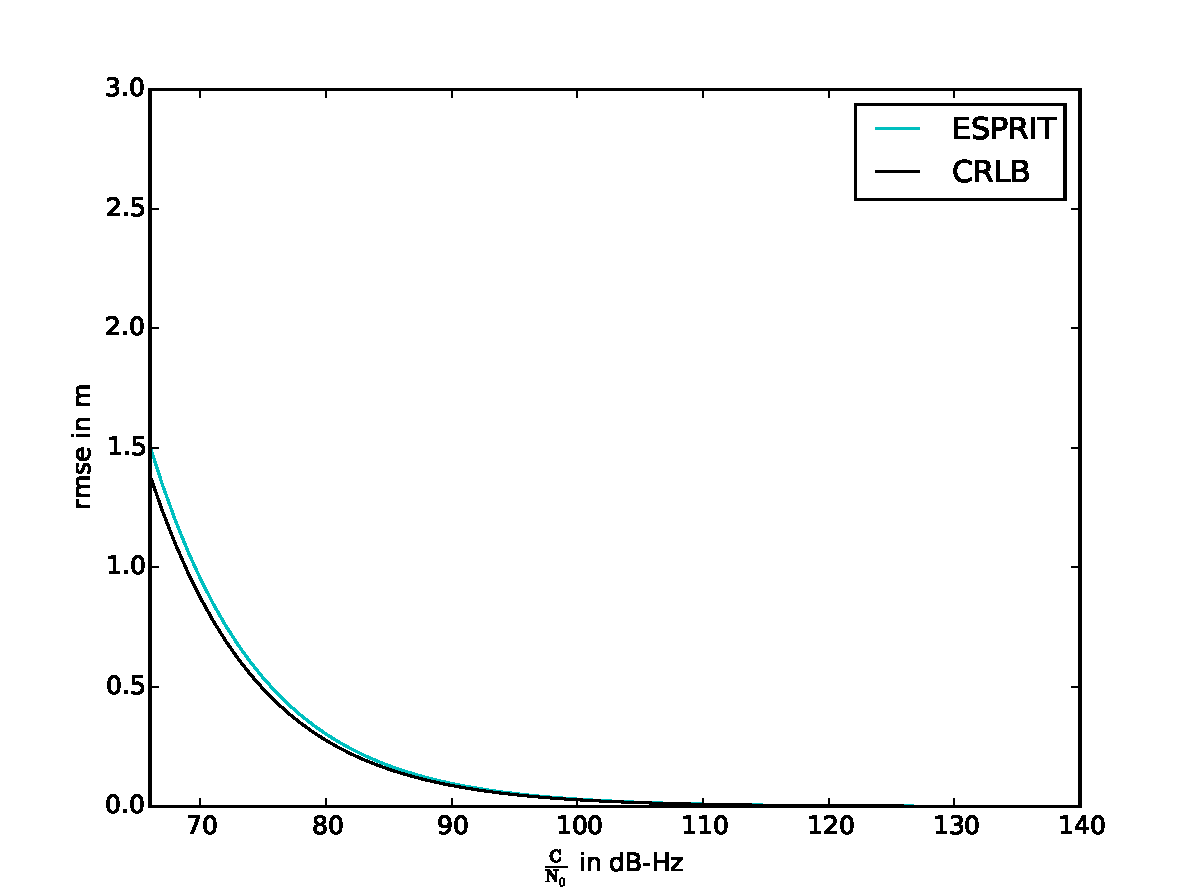
\includegraphics[width = 0.5\textwidth]{images/ESPRIT_7Ton_CRLB}} &
		\subfloat[1025-Ton]{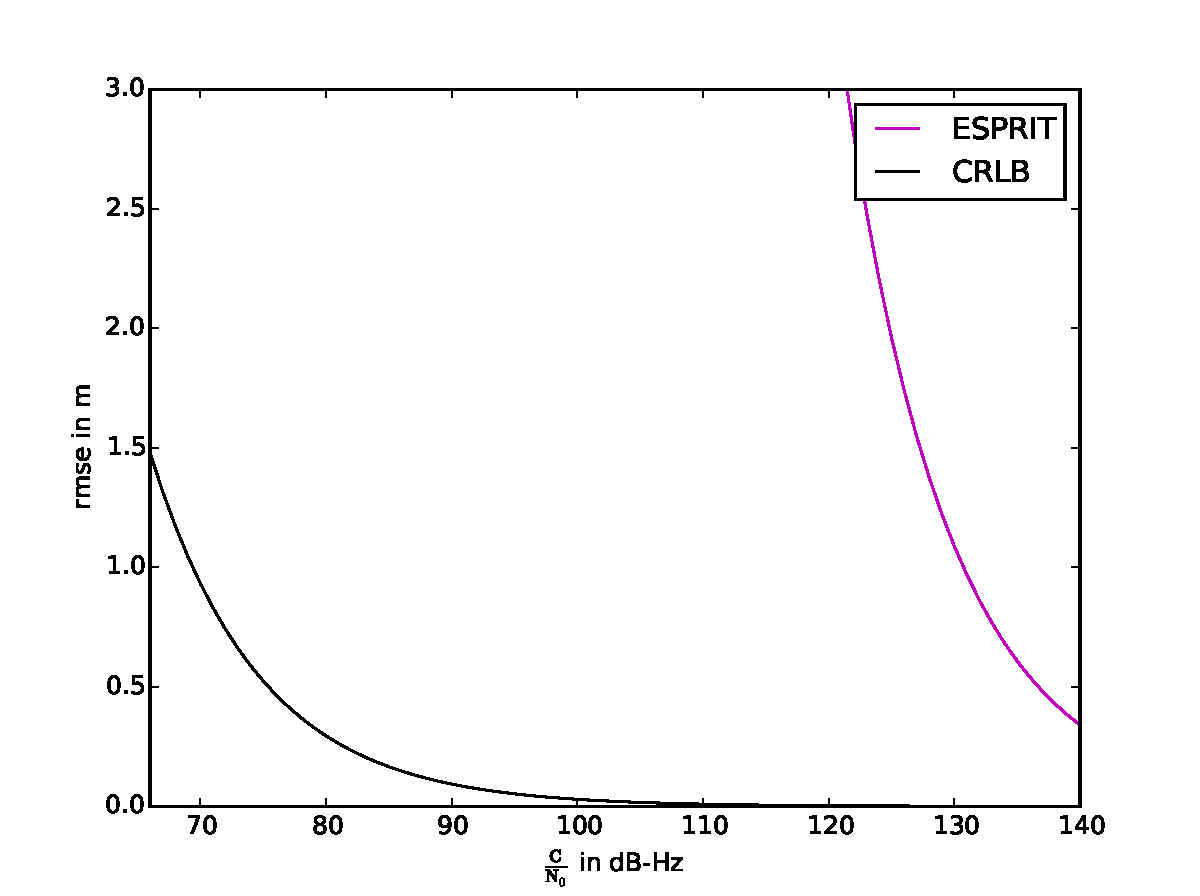
\includegraphics[width = 0.5\textwidth]{images/ESPRIT_1023Ton_CRLB}}	
	\end{tabular}}
	\caption{Varianz des \gls{ESPRIT}-Schätzers gegenüber der CRLB für $m$-Sequnzen}
	\label{fig:m_ESPRIT_CRLB_vergleich}
\end{figure}

Wie bereits festgestellt haben die Fehlerkurven des \gls{MUSIC}-Algorithmus einen ähnlichen Verlauf, wie die bei \gls{ESPRIT}. An der Abbildung \ref{fig:MUSIC_CRLB_vergleich} ist jedoch zu erkennen, dass sie etwas näher an der \gls{CRLB} liegen.  

\begin{figure}[htbp]
	\centering
	\makebox[\textwidth][c]{
	\begin{tabular}{cccc}	
		\subfloat[4-Ton]{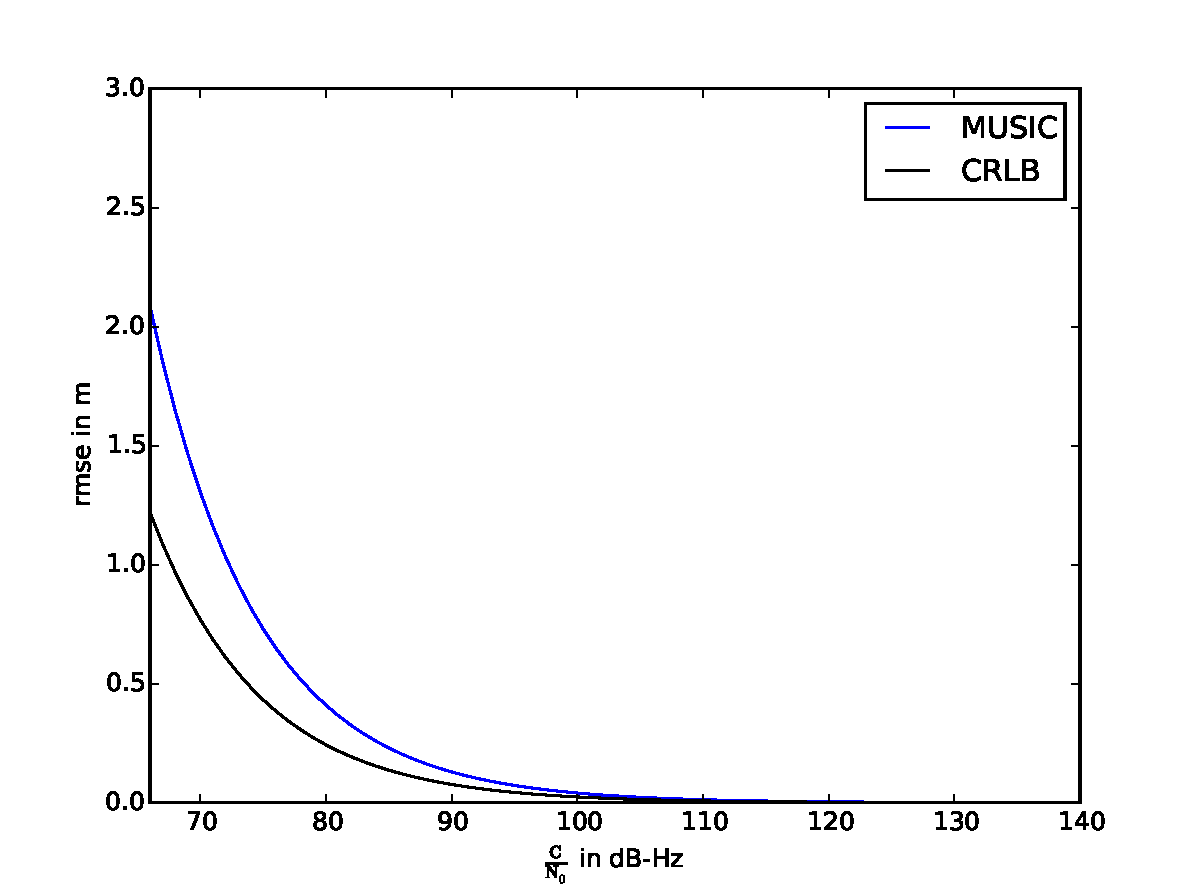
\includegraphics[width = 0.5\textwidth]{images/MUSIC_4Ton_CRLB}} &
		\subfloat[8-Ton]{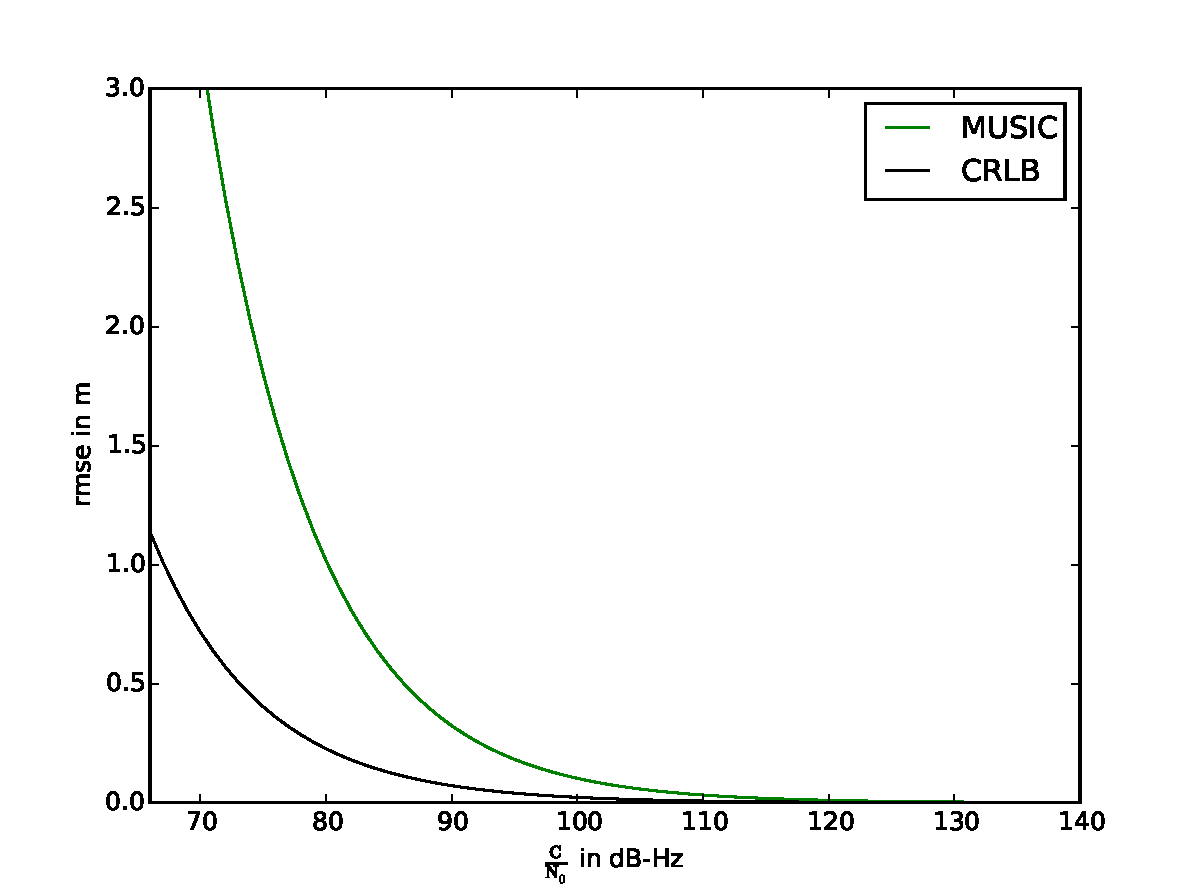
\includegraphics[width = 0.5\textwidth]{images/MUSIC_8Ton_CRLB}} \\		
		\subfloat[16-Ton]{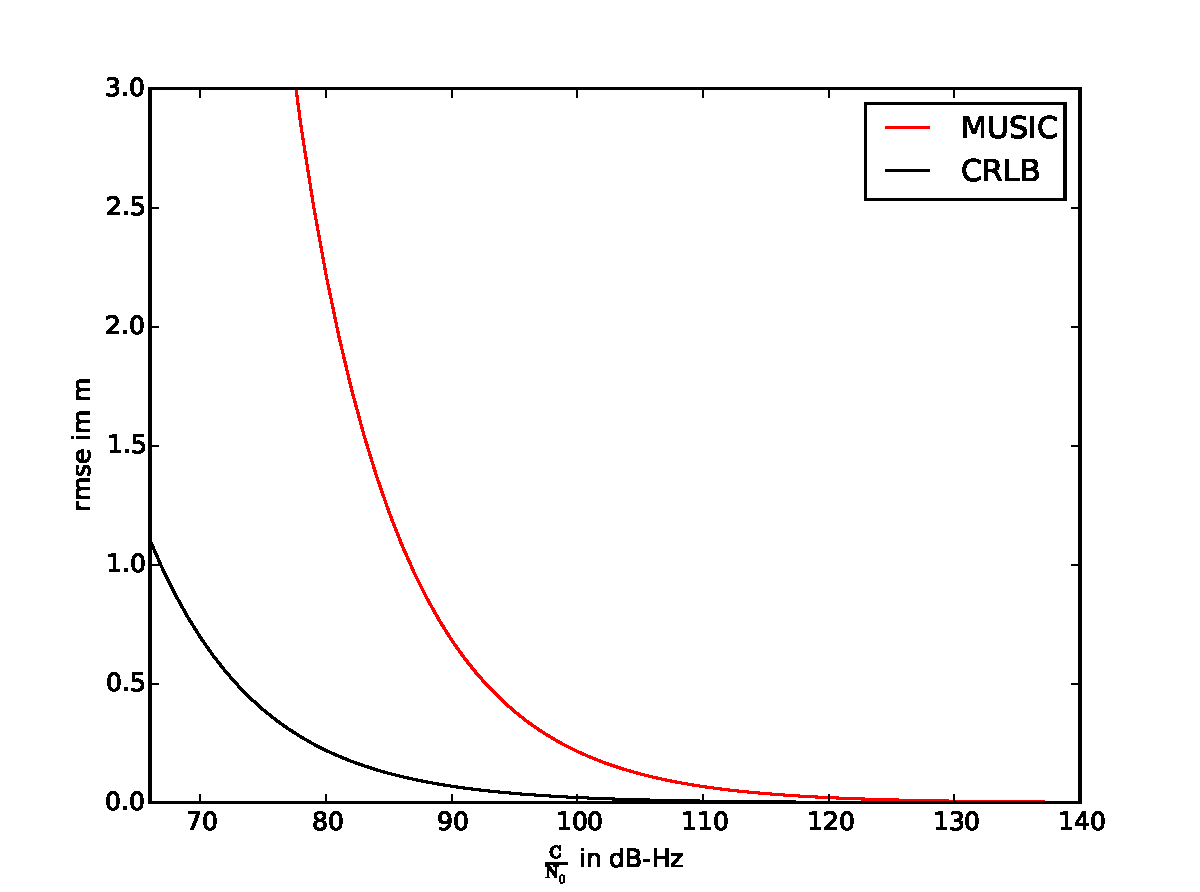
\includegraphics[width = 0.5\textwidth]{images/MUSIC_16Ton_CRLB}} &
		\subfloat[7-Ton]{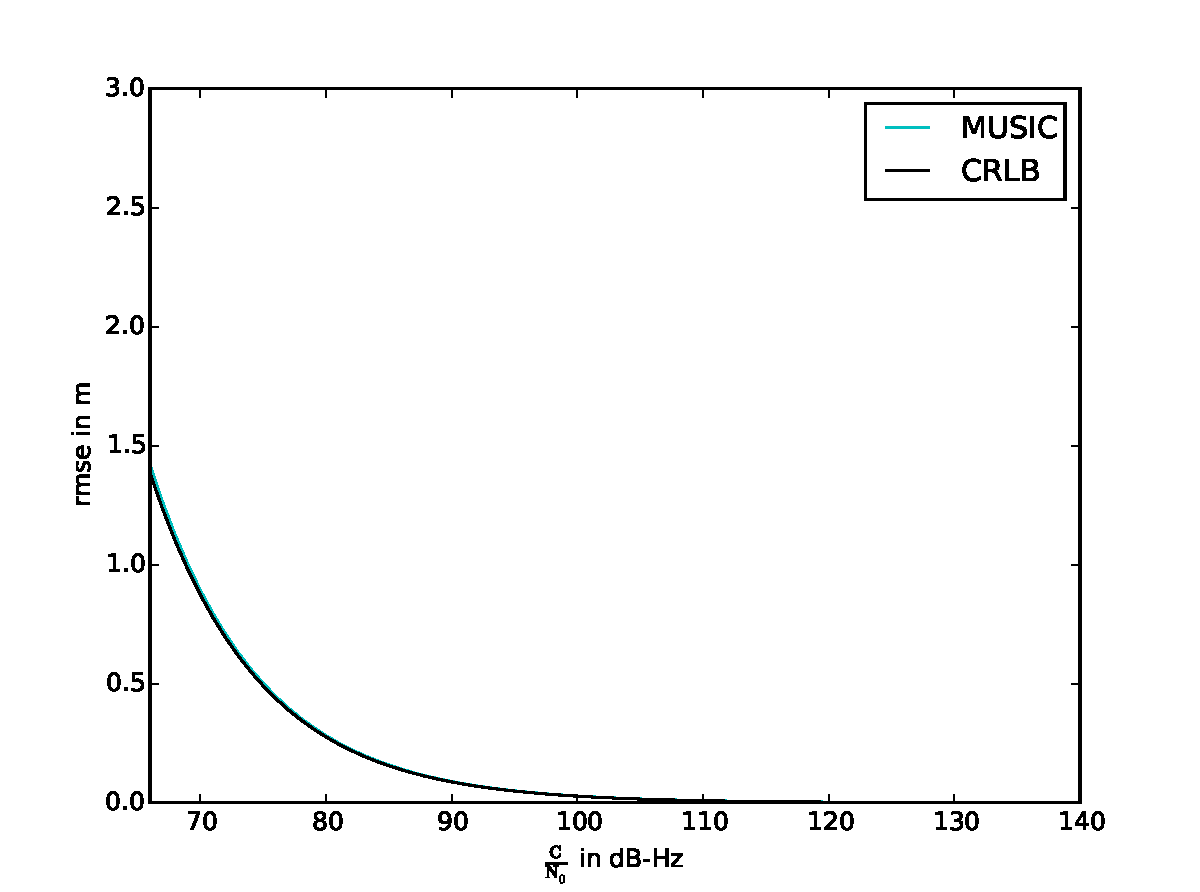
\includegraphics[width = 0.5\textwidth]{images/MUSIC_7Ton_CRLB}}
		\end{tabular}}		
	\caption{Varianz des \gls{MUSIC}-Schätzers gegenüber der \gls{CRLB}}
	\label{fig:MUSIC_CRLB_vergleich}
\end{figure}

Aufgrund der vorangegangenen Auswertungen der Subraummethoden kann geschlussfolgert werden, dass der 7-Ton die einzige Signalform ist, welche mit diesen Verfahren gute Ergebnisse erzielt. Dies lässt sich auch aus der Schätzeffizienz dieser Schätzverfahren für die unterschiedlichen Signale, wie in Abbildung \ref{fig:Schätzeffizienz_Subraum} ablesen. Bei beiden Algorithmen hat der 7-Ton die höchste Effizienz. \gls{MUSIC} übertrifft jedoch \gls{ESPRIT} minimal.

\begin{figure}[htbp]
	\centering
	\makebox[\textwidth][c]{\begin{tabular}{ccc}
		\subfloat[\gls{ESPRIT}]{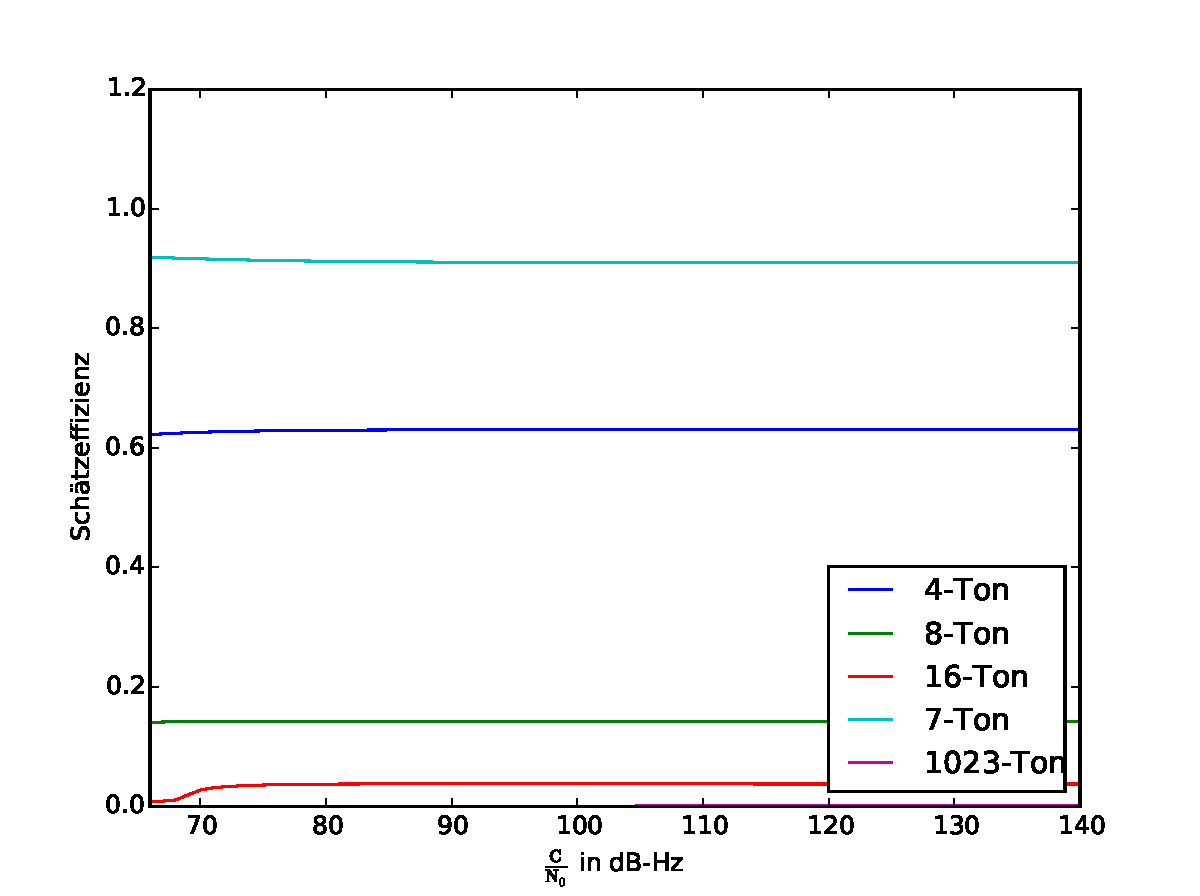
\includegraphics[width = 0.5\textwidth]{images/Schaetzeffizienz_ESPRIT}} &
		\subfloat[\gls{MUSIC}]{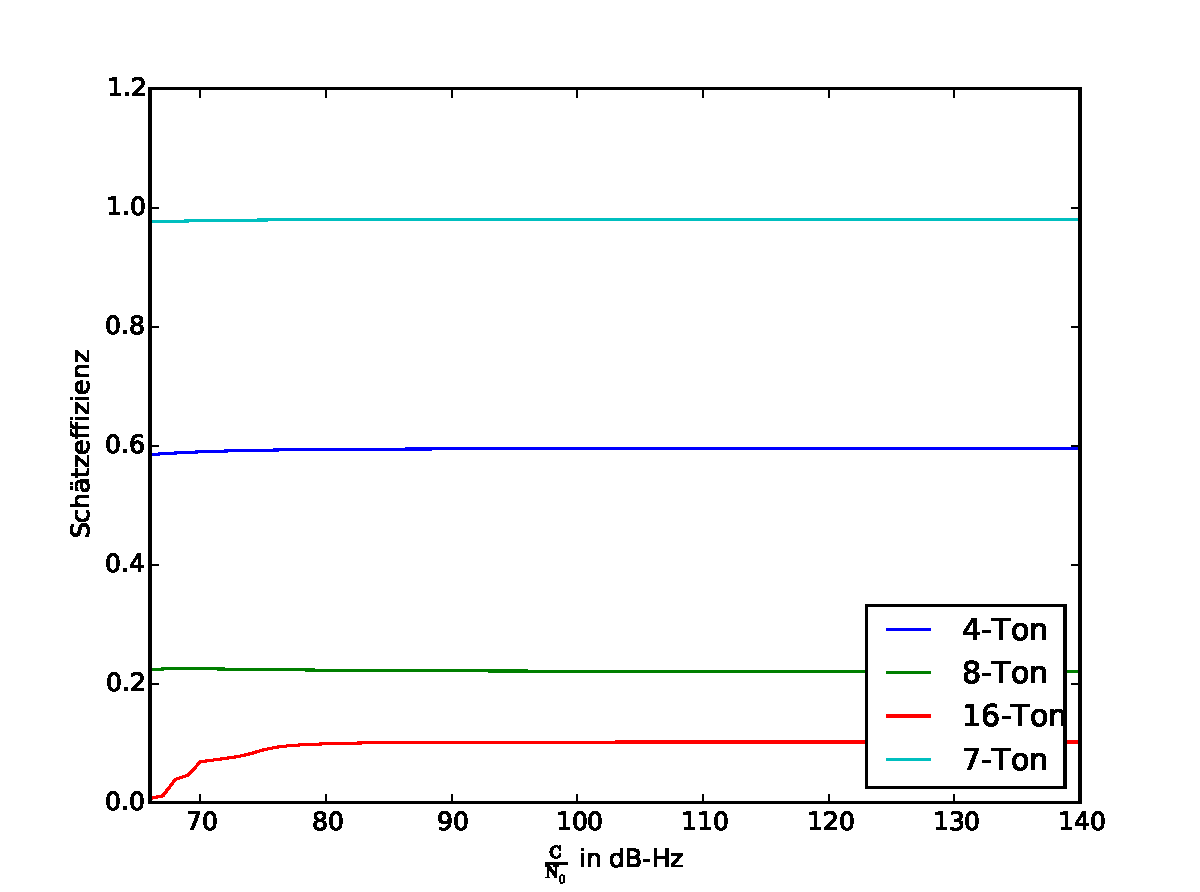
\includegraphics[width = 0.5\textwidth]{images/Schaetzeffizienz_MUSIC}}
	\end{tabular}}
	
	\caption{Schätzeffizienz der Subraumalgorithmen}
	\label{fig:Schätzeffizienz_Subraum}	
\end{figure}



\subsection{Auswertung für den \gls{AWGN}-Fall}

Der gemittelte-Phasendifferenz-Schätzer ist stark von der Energieverteilung auf die jeweiligen Subträger abhängig und macht bei einem fast weißen Spektren einen sehr großen Fehler. Der \gls{LuR}-Schätzer schafft es allerdings gerade bei diesen Sequenzen das \nicefrac[]{\gls{symb:C}}{\gls{symb:N0}} erheblich zu verbessern und ist daher im \gls{AWGN}-Fall deutlich weniger fehleranfällig. Ein großer Nachteil des \gls{LuR}-Schätzers, ist jedoch eine Vereinfachung, die getroffen wird, welche bei Hadamard-Sequenzen nicht angewendet werden kann. Gerade diese Sequenzen haben aber besonders gute Eigenschaften um Fehler im \gls{AWGN}-Kanal zu minimieren.
Zusätzlich stellt sich die Impulsformung mit einem Rechteck auch als suboptimal für diesen Schätzer heraus. Um die Stärken des \gls{LuR}-Schätzers voll auszuschöpfen, müssen Signale erzeugt werden, die auch nach der Impulsformung gleich gewichtete Subträger besitzen.    
Auch die Subraummethoden haben Schwierigkeiten mit den Hadamard-Sequenzen, da ein ähnlicher Fehler wie beim \gls{LuR}-Schätzer gemacht wird. Anders als beim \gls{LuR}-Schätzer können die schlechten \gls{AWGN}-Eigenschaften des 1023-Tons nicht verbessert werden und führen dementsprechend zu großen Fehlern bei kleinen \nicefrac[]{\gls{symb:C}}{\gls{symb:N0}}. Am besten funktionieren die Subraummethoden mit einem 7-Ton. 

\section{Betrachtung bei Mehrwegeausbreitung}
\label{chap5.2:Mehrwege}
In Abschnitt \ref{chap2.3.3:Hüllkurven} wurde bereits diskutiert, dass die \gls{CRLB} kein sinnvolles Maß zum quantifizieren eines Schätzer unter Einfluss eines Mehrwegekanals ist. An ihrer Stelle werden Fehlerhüllkurven erzeugt, um das, von unterschiedlichen Parametern abhängige, Verhalten der Schätzer genauer zu untersuchen. Diese Hüllkurven erlauben es zwar nicht, eine Aussage darüber zu treffen, ob ein Schätzer der Bestmögliche hinsichtlich eines \gls{mvue} ist, sie geben aber Aufschluss darüber, ob die Schätzer untereinander Vor- oder Nachteile aufweisen. Zudem kann eine Aussage darüber getroffen werden, ob die Fehler, die entstehen können, in einem realen System zu tolerieren sind. Der untersuchte Mehrwegekanal besteht aus zwei Pfaden. Der Zweite Pfad hat den Betrag $\alpha = 0,5$. Diese Annahme legt das Verhältnis des \gls{SNR} vom \gls{LOS} zum \gls{SNR} des Umwegpfad fest, was jedoch realitätsfern ist. Das \gls{SNR} des Umwegpfades ist in der Realität distanzabhängig. Die Annahme vereinfacht jedoch das Modell und liefert allgemeine Erkenntnisse und Tendenzen über das Mehrwegeauflösungsvermögen der Schätzer.

\subsection{Auswertung des gemittelten-Phasendifferenz-Schätzers}
\label{chap:5.2.1:gemittelte Phasendifferenz}
Zunächst sollen die Hüllkurven im Basisband betrachtet werden, um anschließend Einflusse der Trägerfrequenz erkennen zu können. 

\begin{figure}[htbp]
	\centering
	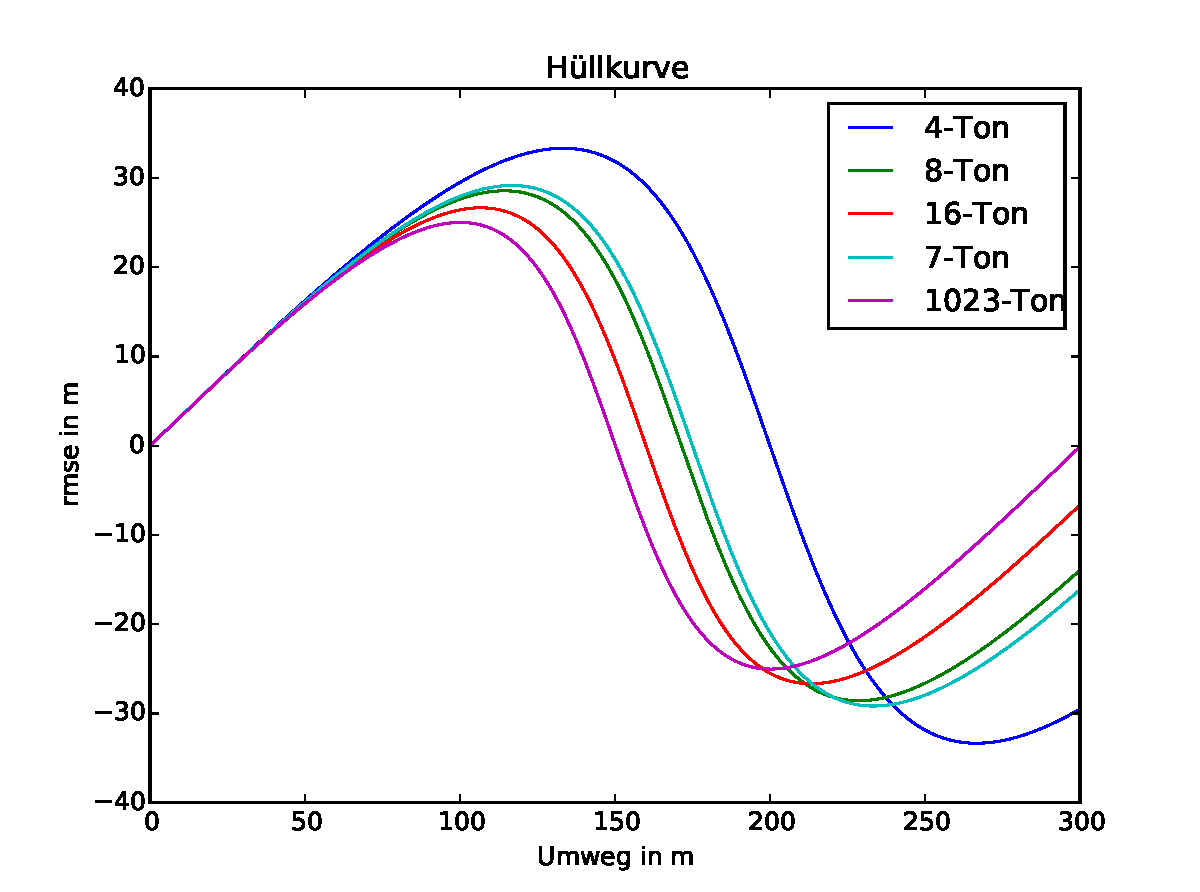
\includegraphics[width = 0.7\textwidth]{images/Huellkurve_ohne_Traeger}
	\caption{Mittlerer Schätzfehler durch einen zweiten Pfad, ohne Einfluss eines Phasenoffsets}
	\label{fig:HullkurveBasisband}
\end{figure}

Streng genommen ist die Abbildung \ref{fig:HullkurveBasisband} keine vollständige Hüllkurve. Erst wenn Phasenoffsets bis $\unit[180]{^\circ}$ berücksichtigt werden, wird die Einhüllende sichtbar. Der besseren Übersichtlichkeit halber werden in dieser Abbildung keine Phasenoffsets abgebildet. Es ist zu erkennen, dass der Fehler sich periodisch über dem Umweg wiederholt. Die Periodendauer wird jedoch mit steigender Subträgerzahl kleiner. Diese Periodizität ist im Abstand zweier benachbarter Abtastwerte begründet, welcher durch $T_{chip}=\nicefrac[]{1}{\gls{symb:B}}$ gegeben ist. Ist das Signal des Umwegpfads um genau einen Abtastwert länger verzögert, als das Signal des \gls{LOS}, haben dessen Subträger eine um $\unit[180]{^\circ}$ verdrehte Phasenlage. Aus Abbildung \ref{fig:MehrwegeZeiger} kann entnommen werden, dass bei einer solchen Phasenlage des Umwegs zum \gls{LOS}, kein Phasenfehler entsteht. Lediglich der Betrag des Umwegs interferiert destruktiv mit dem \gls{LOS}. Deshalb durchläuft die Kurve an dieser Stelle den Nullpunkt. Um die Unterschiede der Periodendauern $T_{chip}$ der Signale zu erklären, müssen die Spektren genauer betrachtet werden. In diesen kann erkannt werden, dass die Bandbreite, je nach Subträgerverteilung variiert. Lediglich die $m$-Sequenz mit 1023 Subträgern hat eine Bandbreite von $\unit[2]{MHz}$ und hat deshalb ihren Nulldurchlauf bei $\unit[150]{m}$.
Des Weiteren ist festzustellen, dass sich der maximale Fehler mit steigender Subträgerzahl verringert. Das zeigt, dass Mehrwegefehler durch Mittelung reduziert werden können. Jedoch liegen diese bei dem Testsignal mit der höchsten Anzahl an Subträgern noch über $\unit[20]{m}$. Ein solcher Fehler in der Distanzschätzung ist für Ortungssysteme nicht tolerabel. 

Als nächstes soll der Einfluss von Phasenoffsets genauer untersucht werden. 
\begin{figure}[htbp]
	\centering
	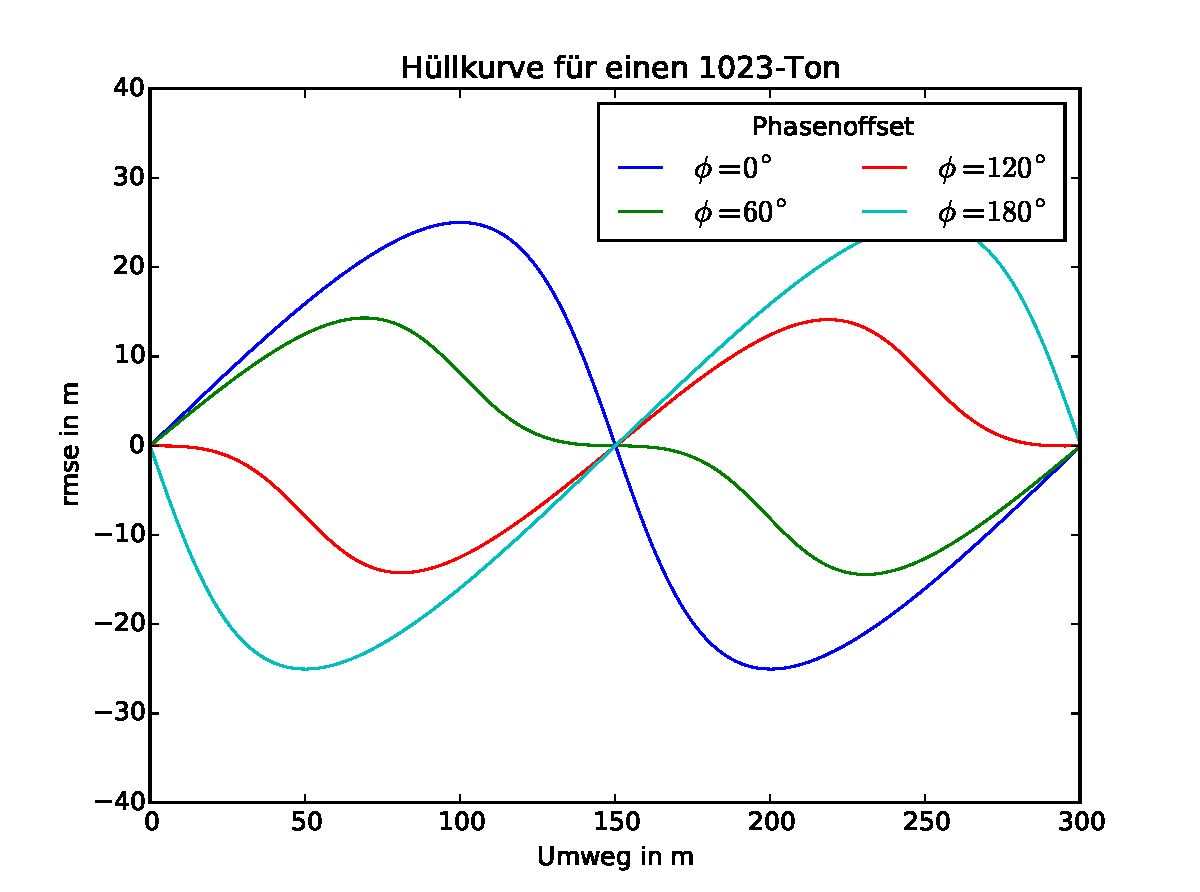
\includegraphics[width = 0.7\textwidth]{images/Hullkurven_1023Ton_ohneTraeger}
	\caption{Hüllkurve einer $m$-Sequenz unter Einfluss von Phasenoffsets}
	\label{fig:Hüllkurve mit Phasenoffset}
\end{figure}
In Abbildung \ref{fig:Hüllkurve mit Phasenoffset} ist eine Hüllkurve für einen 1023-Ton und vier Phasenoffsets zu sehen. Es ist zu erkennen, dass durch zufällige Phasendrehungen, durch Objekte an denen das Signal des zweite Pfad reflektiert wird, die maximalen Fehler zwischen den Fehlerkurven für $\unit[0]{^\circ}$ und $\unit[180]{^\circ}$ liegen. Wenn die Trägerfrequenz \gls{symb:fc} mitberücksichtigt wird, verändern sich die Hüllkurven jedoch leicht. 

\begin{figure}[htbp]
	\centering
	\makebox[\textwidth][c]{\begin{tabular}{cccc}
		\subfloat[4-Ton]{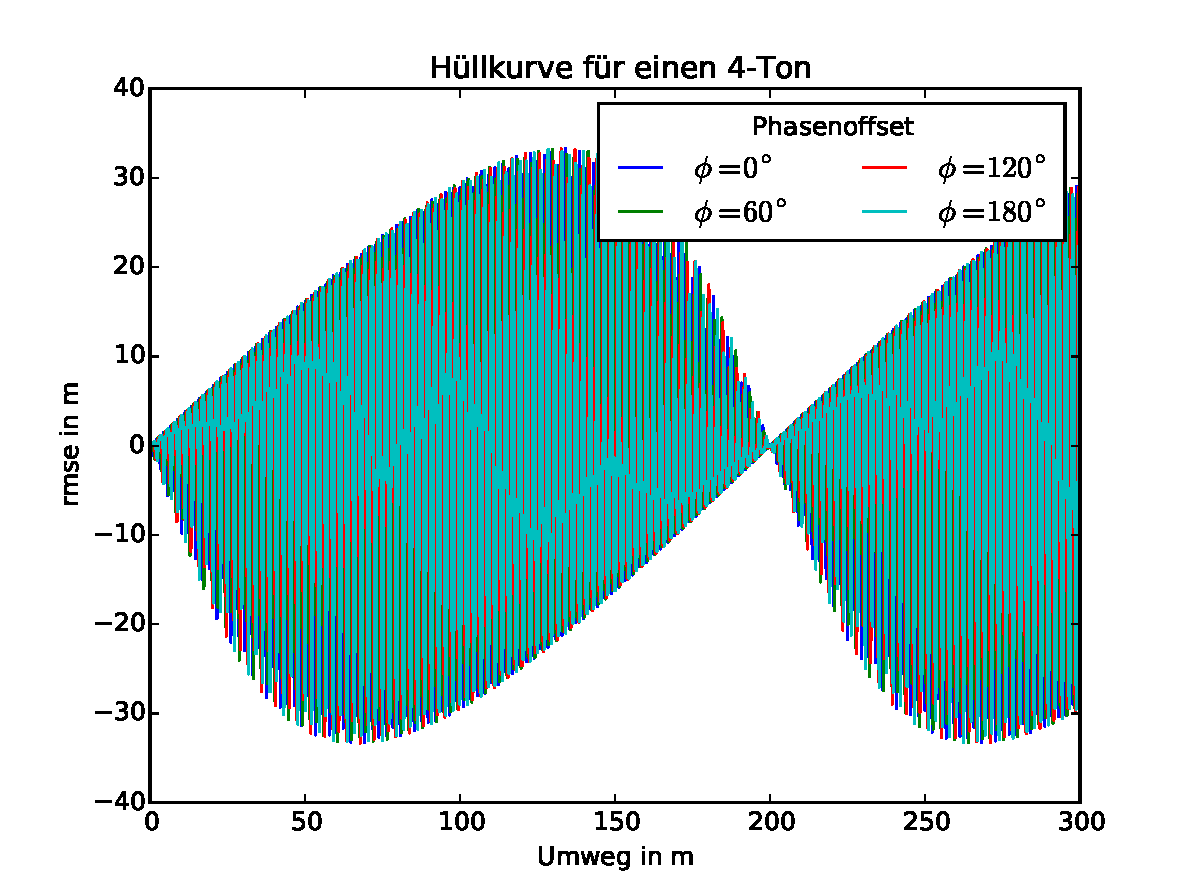
\includegraphics[width = 0.5\textwidth]{images/Hullkurven_4_Ton}} &
		\subfloat[16-Ton]{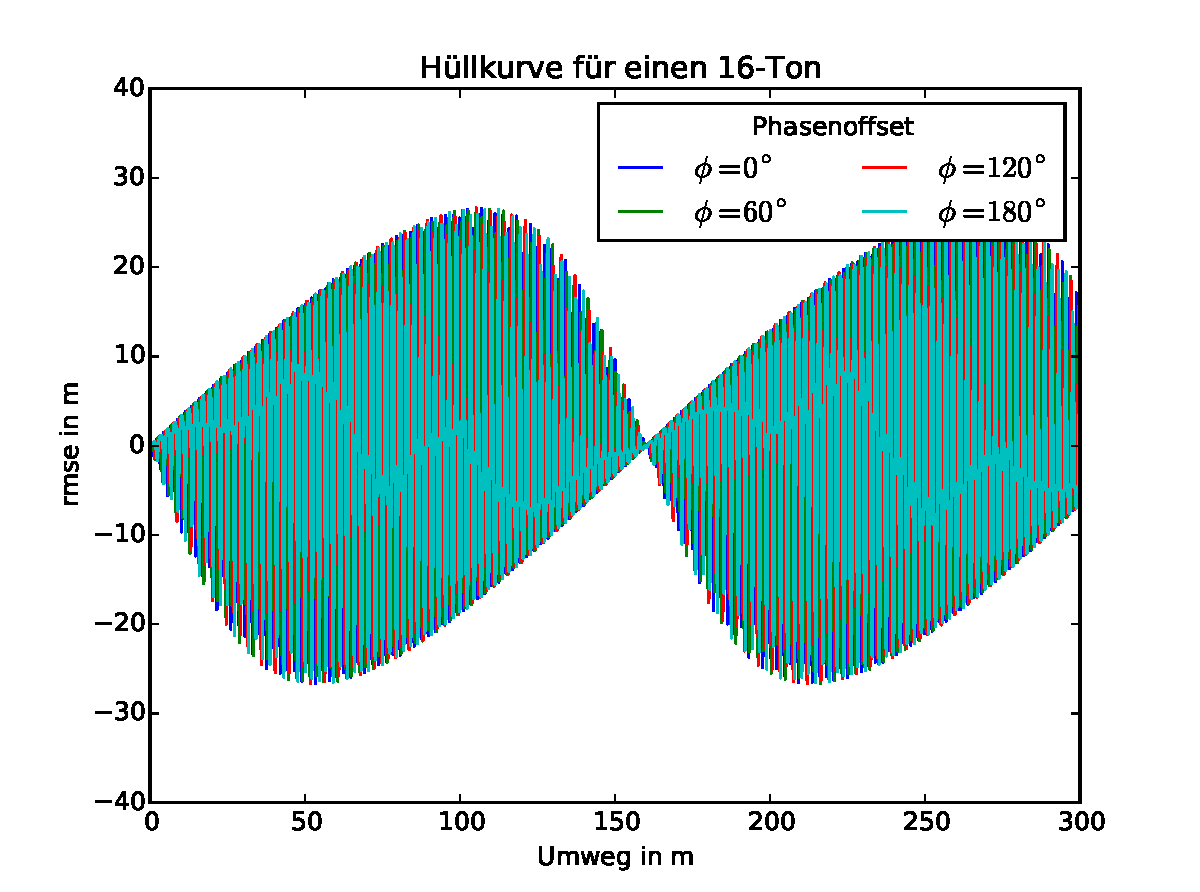
\includegraphics[width = 0.5\textwidth]{images/Hullkurven_16_Ton}}
	\end{tabular}}
	\caption{Hüllkurven zweier Hadamard-Sequenzen mit einer Trägerfrequenz \gls{symb:fc}$=\unit[868]{MHz}$ und unter Einfluss von Phasenoffsets}
	\label{fig:Hüllkurve mit Träger}
\end{figure}	

Der Zeiger des Umwegpfades aus Abbildung \ref{fig:MehrwegeZeiger} dreht sich aufgrund der Trägerfrequenz nun deutlich schneller. Dadurch umrundet dieser Zeiger für jeden gewanderten Meter etwa $2,8$ mal die Spitze des \gls{LOS}-Zeigers. Diese Periodizität von ungefähr $\unit[35]{cm}$ ist in Abbildung \ref{fig:Hüllkurve mit Träger} deutlich zu erkennen. Es ist ersichtlich , dass sich am maximalen Mehrwegefehler nichts geändert hat. Jedoch scheinen die Phasenoffsets keinen großen Einfluss mehr auf diesen zu haben. Um das genauer untersuchen zu können, ist im Folgenden eine Vergrößerung der Abbildung \ref{fig:Hüllkurve mit Träger} zu sehen. 

\begin{figure}[htbp]
	\centering
	\makebox[\textwidth][c]{\begin{tabular}{cccc}
		\subfloat[4-Ton]{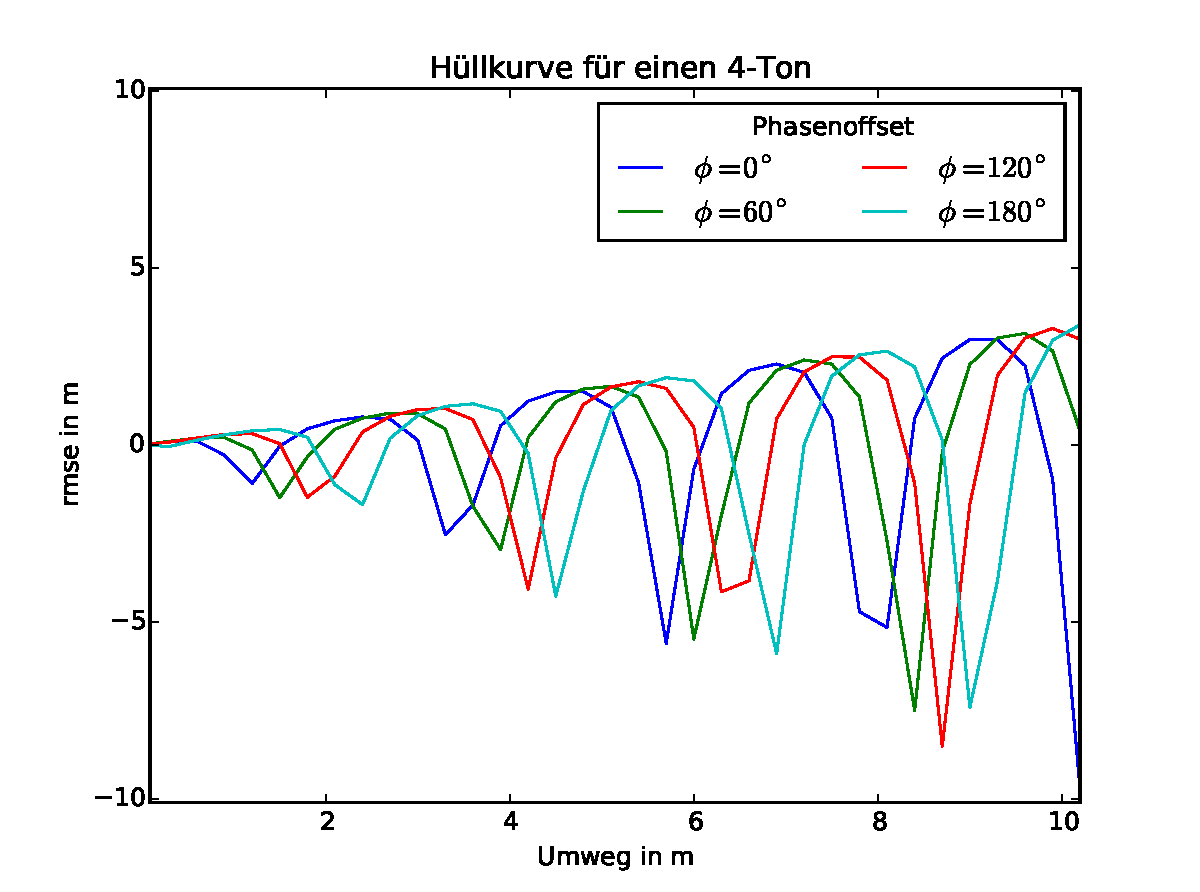
\includegraphics[width = 0.5\textwidth]{images/Hullkurven_4_Ton_zoom}} &
		\subfloat[16-Ton]{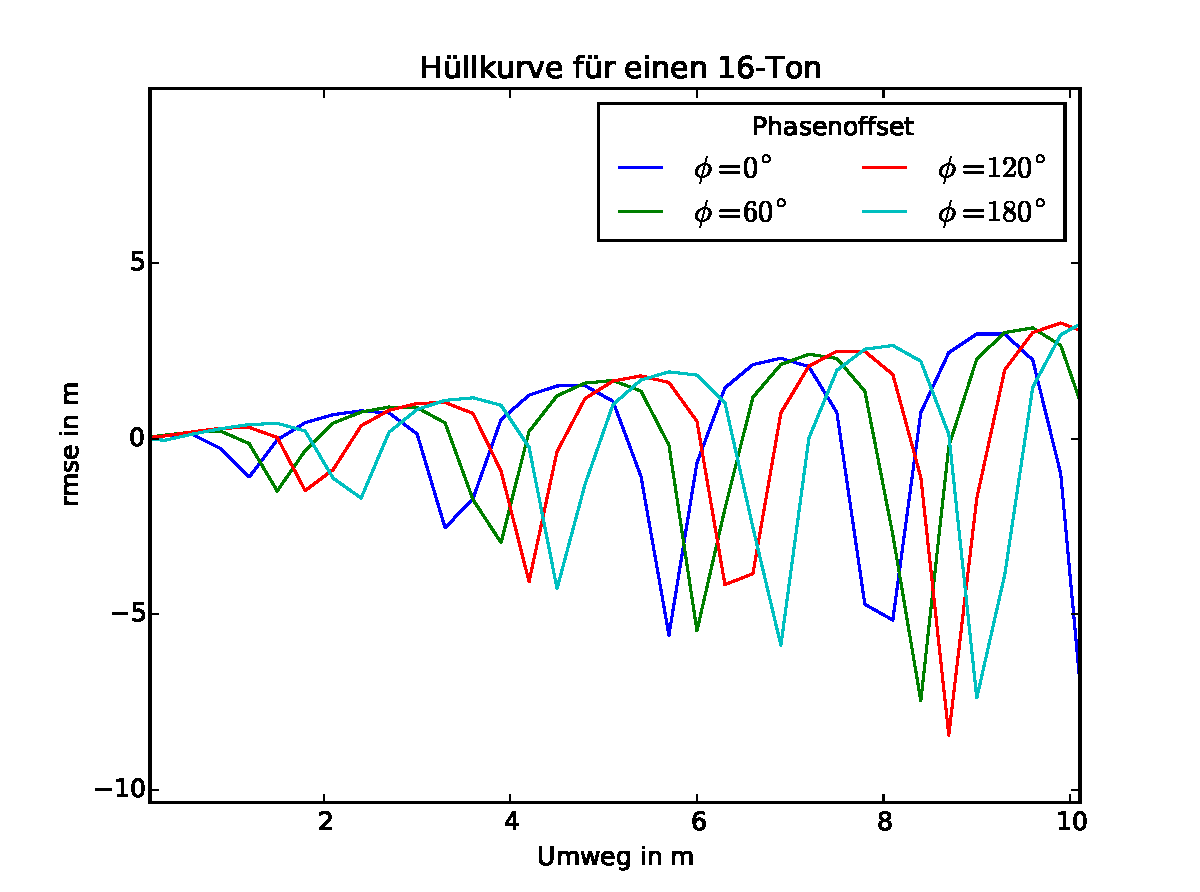
\includegraphics[width = 0.5\textwidth]{images/Hullkurven_16_Ton_zoom}}
	\end{tabular}}
	\caption{Hüllkurven zweier Hadamard-Sequenzen mit einer Trägerfrequenz von $\unit[868]{MHz}$ und unter Einfluss von Phasenoffsets}
	\label{fig:Hüllkurve mit Träger gezoomt}
\end{figure}

Anhand dieser Vergrößerungen wird sichtbar, dass die Fehlerkurven später einsetzen. Somit verschiebt der Phasenoffset die Kurven nur und beeinflusst den maximalen Fehler nicht. 


\subsection{Auswertung des \gls{LuR}-Schätzers}

Beim \gls{LuR}-Schätzer war die Annahme, dass, durch Verwendung unterschiedlicher Abstände zwischen den Subträgern, zur Phasendifferenzbildung eine höhere Genauigkeit erzielt werden kann. Im Abschnitt \ref{chap5.1.2:LundR Auswertung} wurde bereits festgestellt, dass dieser Schätzer eine suboptimale Vereinfachung trifft, welche nicht auf die hier verwendeten Signale zutrifft. Dadurch müssen alle Subträger im Schätzer zunächst skaliert werden. Folglich wird auch der Mehrwegefehler, mit denen die Subträger vorher behaftet sind, skaliert. Es stellt sich die Frage, wie sich diese Maßnahme auf die Hüllkurven auswirkt. Zunächst wird jedoch, wie in Abschnitt \ref{chap:5.2.1:gemittelte Phasendifferenz} der mittlere Schätzfehler bei Mehrwegeausbreitung ohne Einfluss von Trägerfrequenz oder Phasenoffsets betrachtet.
 
\begin{figure}[htbp]
	\centering
	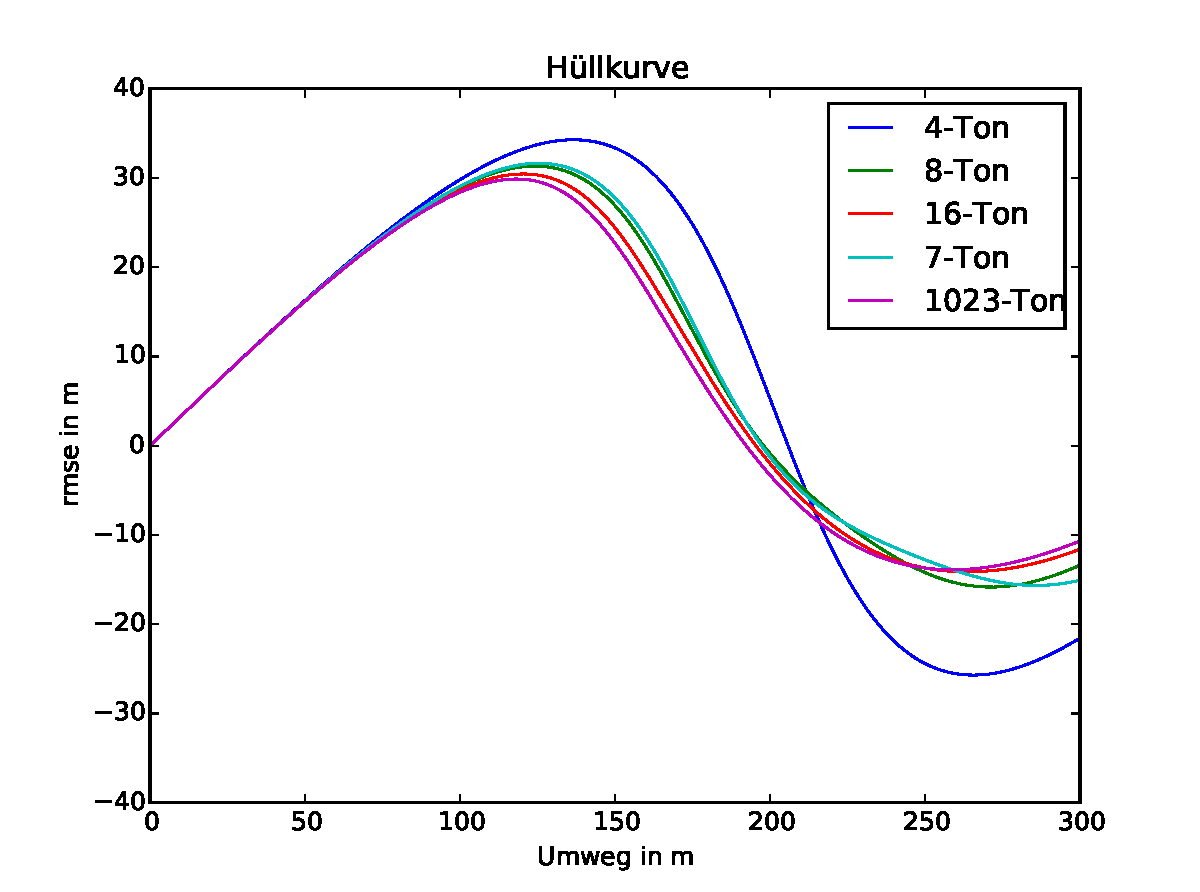
\includegraphics[width = 0.7\textwidth]{images/LuR_Huellkurve_ohne_Traeger}
	\caption{Mittlerer Schätzfehler durch einen 2. Pfad, ohne Einfluss eines Phasenoffsets}
	\label{fig:LuRHullkurveBasisband}
\end{figure}

Die Periodendauer des Fehlers der unterschiedlichen Signale wird bei diesem Schätzer nicht kleiner. Dies deutet schon auf ein fehlerhaftes Verhalten des Schätzers hin. 
Der maximale Fehler dieses Schätzverfahrens nimmt zwar auch mit zunehmender Subträgerzahl ab, verglichen mit dem gemittelten-Phasendifferenz-Schätzer, jedoch in einem viel geringerem Maß. Zwischen 8-Ton und 1023-Ton ist kaum noch eine Verbesserung zu sehen. Die getroffenen Maßnahmen, um diesen Schätzer an die Signale anzupassen, scheinen die Leistungsfähigkeit beeinträchtigt zu haben. Nicht nur an der Lage des Nulldurchlaufs der Kurven für die Signale, sondern auch an den Kurven mit Phasenoffsets, kann ein ungewöhnliches Verhalten des Schätzfehlers festgestellt werden. In Abbildung \ref{fig:LuRHüllkurve mit Phasenoffset} ist zu erkennen, dass die Periodendauer des Fehlers für unterschiedliche Phasenoffsets nicht bei den selben Verzögerungen liegen, wie es beim gemittelten-Phasendifferenz-Schätzers der Fall war. In Abbildung \ref{fig:HüllkurvenLuR-Had} ist an dieser Stelle eine Verzerrung zu sehen.

\begin{figure}[htbp]
	\centering
	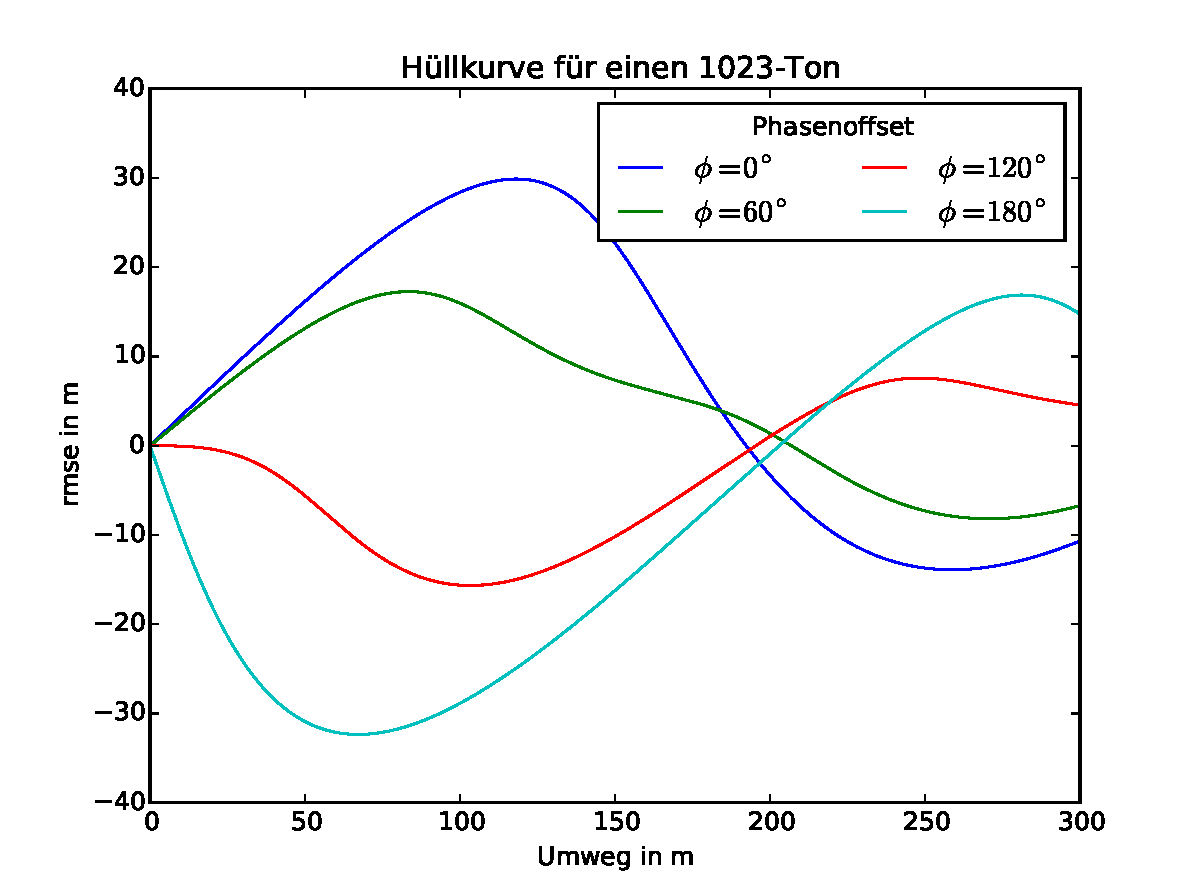
\includegraphics[width = 0.7\textwidth]{images/LuR_Hullkurven_1023_ohneTraeger}
	\caption{Hüllkurve einer m-Sequenz unter Einfluss von Phasenoffsets}
	\label{fig:LuRHüllkurve mit Phasenoffset}
\end{figure}
 
Eine weitere Beobachtung ist, dass der maximale \gls{rmse} in der zweiten Periode kleiner wird. Sehr deutlich kann dieser Effekt bei dem 1023-Ton, in Abbildung \ref{fig:LuRHüllkurve mit Phasenoffset} erkannt werden. Die Begründung hierfür ist der zu lange Umwegpfad. Der \gls{LuR}-Schätzer hat einen deutlich kleineren Eindeutigkeitsbereich als der gemittelte-Phasendifferenz-Schätzer, sodass der Umwegpfad diesen nach der ersten Periode verlässt.

\begin{figure}
	\makebox[\textwidth][c]{\begin{tabular}{ccc}
		\subfloat[4-Ton]{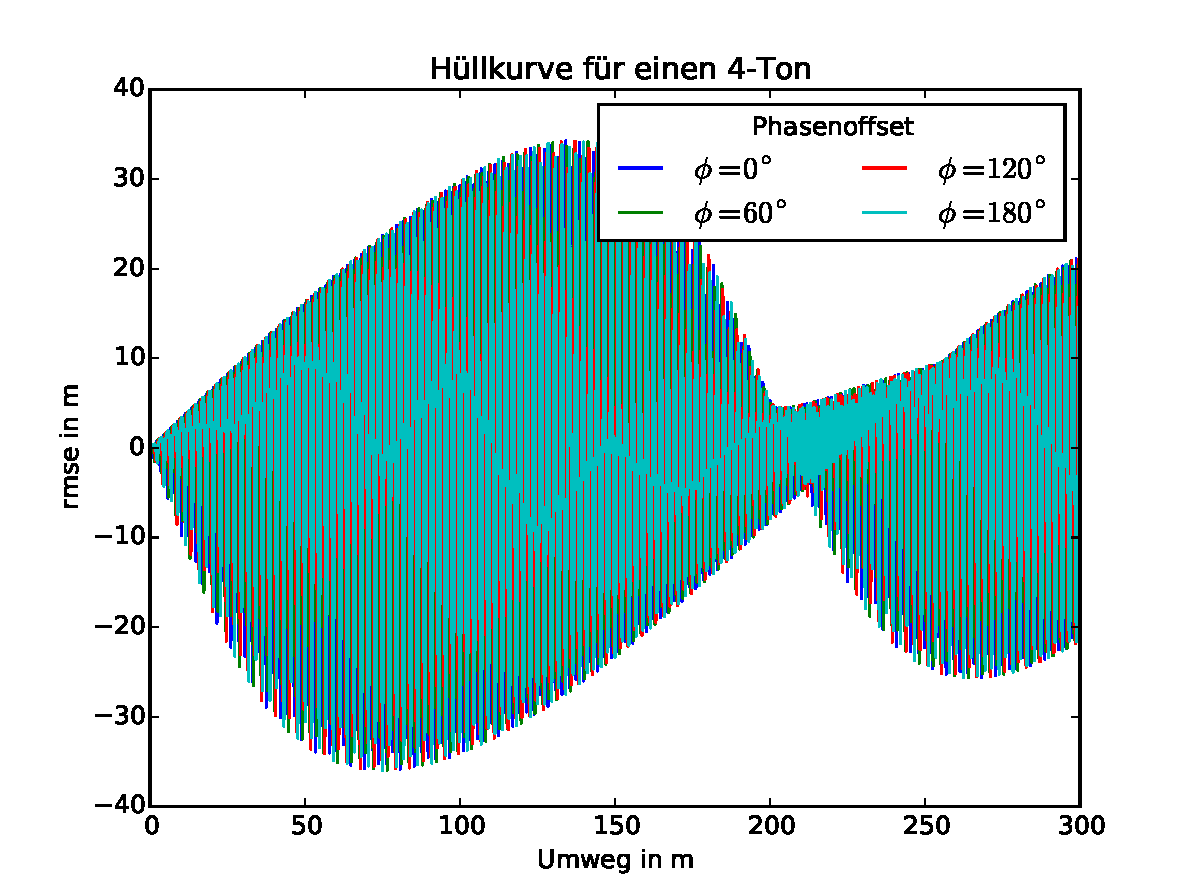
\includegraphics[width = 0.5\textwidth]{images/Hullkurven_4_LuR}} &
		\subfloat[16-Ton]{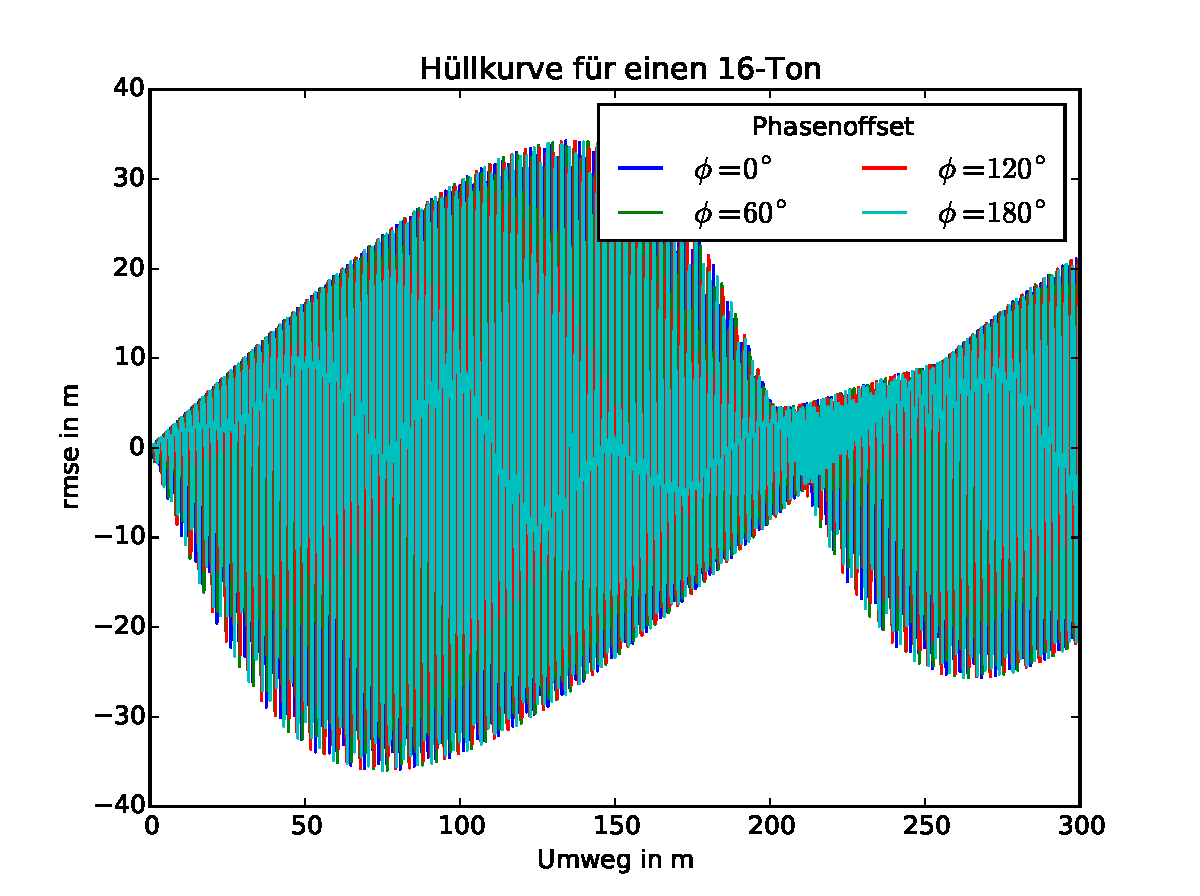
\includegraphics[width = 0.5\textwidth]{images/Hullkurven_16_LuR}}
		\end{tabular}}
		\caption{Hüllkurven des \gls{LuR} Schätzers}
		\label{fig:HüllkurvenLuR-Had}
\end{figure}				

Dieser Schätzer liefert für die hier verwendeten Signale kein besseres Auflösungsvermögens des Mehrwegekanals. Um bessere Ergebnisse zu erzielen, müssen Signale verwendet werden, die die Bedingungen für das Verwenden der Gleichung \eqref{eq:Approximation} erfüllen. Die nachträgliche Skalierung der Subträgergewichte führt zu einem unerwarteten Verhalten.  

\subsection{Auswertung der Subraumalgorithmen}

Wie bereits im \gls{AWGN}-Fall erwähnt, liefern \gls{MUSIC} und \gls{ESPRIT} ähnliche Ergebnisse. 
\begin{figure}
	\makebox[\textwidth][c]{\begin{tabular}{ccc}
		\subfloat[4-Ton]{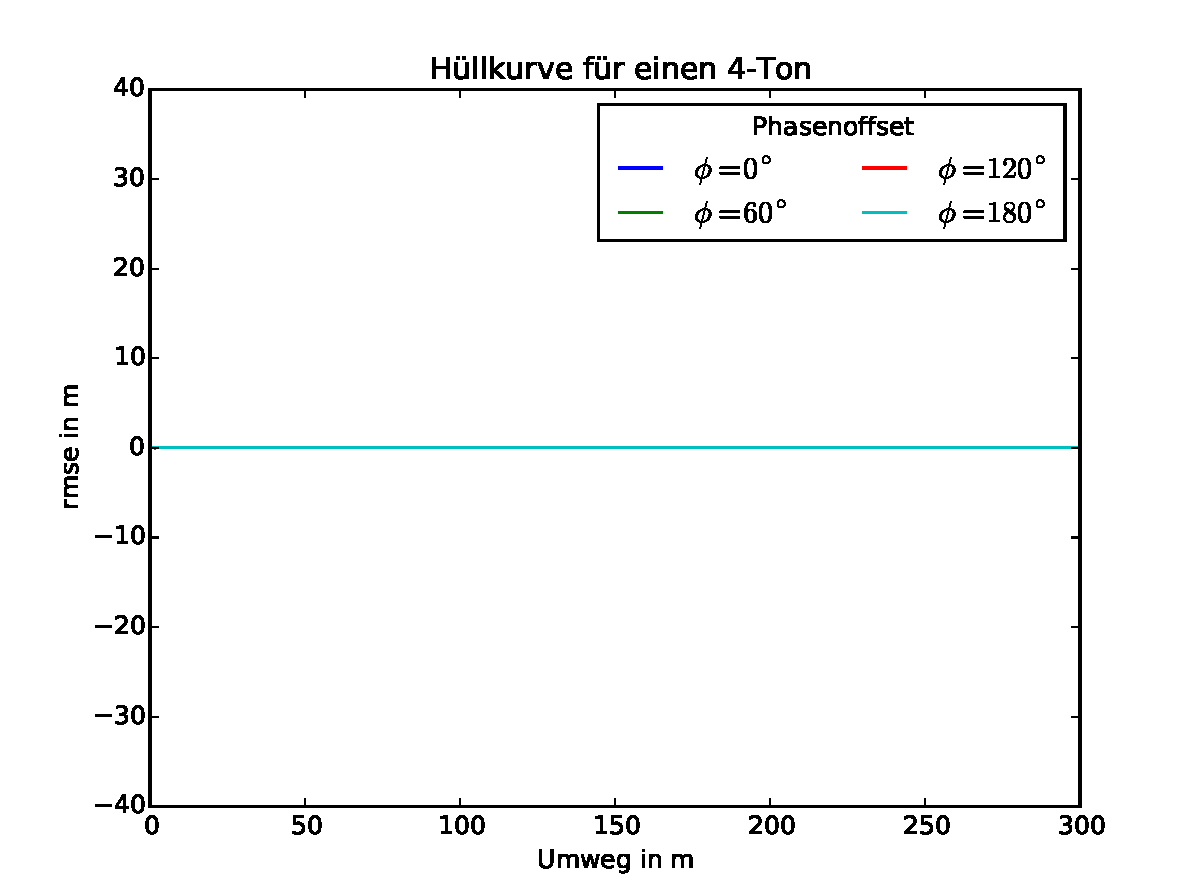
\includegraphics[width = 0.5\textwidth]{images/Hullkurven_4Ton_ESPRIT}} &
		\subfloat[7-Ton]{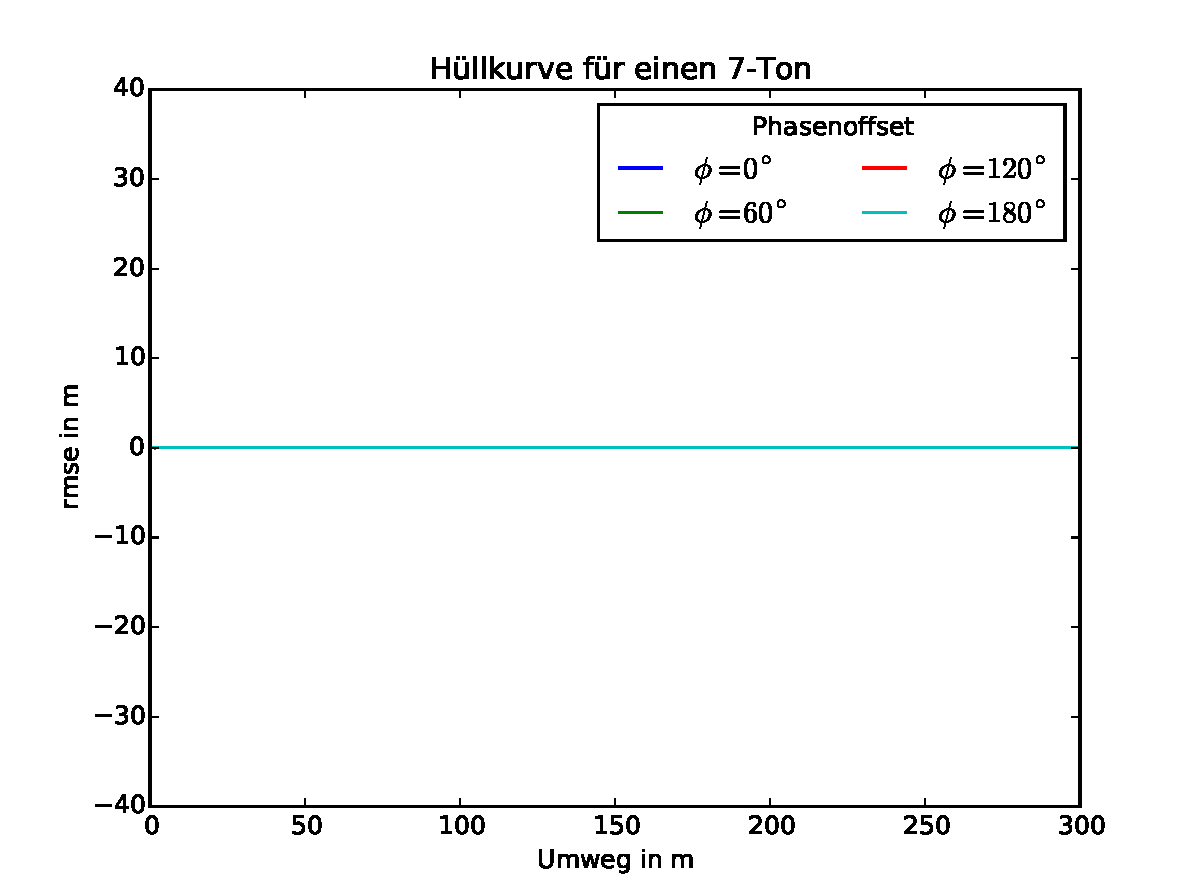
\includegraphics[width = 0.5\textwidth]{images/Hullkurven_7Ton_ESPRIT}}
	\end{tabular}}
	\caption{Mehrwegehüllkurven einer Hadamard- und einer $m$-Sequenz}
	\label{fig:ESPIT_Mehrwege}
\end{figure}
Da diese Algorithmen die Pfade trennen können, ist es nicht weiter verwunderlich, dass bei Mehrwegeausbreitung kein Schätzfehler entsteht, wie in Abbildung \ref{fig:ESPIT_Mehrwege}. 
Es stellt sich jedoch die Frage, ob diese Eigenschaft, die Pfade trennen zu können, auch bei schlechten Signal-Rausch-Verhältnissen bestehen bleibt. 

\subsection{Bewertung bei Mehrwegeausbreitung}
In den vorangegangenen Auswertungen stellte sich heraus, dass Mittelungsverfahren den Schätzfehler in einem Mehrwegekanal durch Mehrtonsignale reduzieren können, jedoch diese immer noch zu groß bleiben. Der maximale Fehler war bei dem gemittelten-Phasendifferenz-Schätzer in Kombination mit der $m$-Sequenz mit 1023 Subträgern am kleinsten, liegt allerdings immer noch über $\unit[20]{m}$. Es hat sich auch herausgestellt, dass der \gls{LuR}-Schätzer, aufgrund seiner Modifikationen für die verwendeten Signale, schlechter als der gemittelte-Phasendifferenz-Schätzer abschneidet. Allerdings zeigt er vielversprechende Tendenzen und sollte nochmals mit geeigneten Signalen und einer geeigneten Impulsformung genauer untersucht werden.    
Die Subraummethoden erweisen sich als die besten Verfahren, Parameter in Mehrwegekanälen zu schätzen. 
Es muss allerdings eine Betrachtung des gesamten Kanals durchgeführt werden, um eine Aussage über die Leistungsfähigkeit zu treffen. 

\section{Betrachtung des gesamten Kanals}
Die Auswertung bei Mehrwegeausbreitung zeigt, dass nur die Subraummethoden handhabbare Fehler produzieren. Mittelungsverfahren, wie sie hier vorgestellt wurden, sind hingegen keine gute Lösung für ein Ortungssystem, dass mehrwegerobust sein soll. 
Zusätzlich stellt sich heraus, dass die $m$-Sequenz mit 7 Subträgern das beste Verhalten bei \gls{AWGN} unter Einsatz der Subraummethoden aufweist. Deshalb soll in diesem Abschnitt der \gls{ESPRIT}- und \gls{MUSIC}-Algorithmus unter Einfluss des gesamten Kanalmodells mit einem 7-Ton untersucht werden. Bei der Untersuchung der Subraummethoden im \gls{AWGN}-Fall konnten Fehler erst ab einem \nicefrac[]{\gls{symb:C}}{\gls{symb:N0}} von $\unit[96]{dB-Hz}$ festgestellt werden. Deshalb wird in den folgenden Betrachtungen der \gls{rmse} für vier \nicefrac[]{\gls{symb:C}}{\gls{symb:N0}}-Werte berechnet. Diese Werte entsprechen den, mit der Bandbreite $\unit[4]{MHz}$ normierten, Signal-Rausch-Verhältnissen $\unit[30]{dB}$, $\unit[20]{dB}$, $\unit[10]{dB}$ und $\unit[0]{dB}$. Im reinen \gls{AWGN}-Fall haben die Algorithmen Fehler im Bereich $\unit[0]{m}-\unit[1,5]{m}$ erzeugt. 

\begin{figure}[htbp]
	\centering
	\makebox[\textwidth][c]{\begin{tabular}{cccc}
		\subfloat[\gls{MUSIC} mit 7-Ton]{\includegraphics[width = 0.5\textwidth]{images/MUSIC_GesamtkanalAuswertung}} &
		\subfloat[\gls{ESPRIT} mit 7-Ton]{\includegraphics[width = 0.5 \textwidth]{images/ESPRIT_GesamtkanalAuswertung}}
	\end{tabular}}
	\caption{Auswertung des Einflusses des gesamten Kanalmodells}
	\label{fig:GesamtkanalAuswertung}
\end{figure}
In Abbildung \ref{fig:GesamtkanalAuswertung} ist der Fehler bei Mehrwegeausbreitung und schlechten Signal-Rausch-Verhältnissen aufgetragen. Man sieht, dass der Fehler nun erheblich größer als im Vergleich zum reinen \gls{AWGN}-Fall geworden ist. Für einen Umwegpfad, länger als $\unit[80]{m}$, flacht der Fehler jedoch wieder ab und liegt sogar bei $\unit[66]{dB-Hz}$ unter $\unit[5]{m}$. Davor kann der maximale Fehler bis zu $\unit[20]{m}$ groß werden. Es ist aber auch zu erkennen, dass alle $\unit[10]{dB-Hz}$, die das \nicefrac[]{\gls{symb:C}}{\gls{symb:N0}} besser wird, der Fehler sich fast halbiert. 
Es zeigt sich, dass bei kurzen Umwegpfaden und schlechten Signal-Rausch-Verhältnissen, die Fehler nicht mehr tolerierbar sind. Verbessert sich jedoch das \nicefrac[]{\gls{symb:C}}{\gls{symb:N0}} um nur $\unit[10]{dB-Hz}$ erreicht man wieder akzeptable Fehlerwerte. Es muss jedoch beachtet werden, dass es Signalformen gibt, welche die Energie, bezüglich einer optimalen \gls{CRLB} noch besser Verteilen könnten. Zudem wird die \gls{CRLB} durch die Impulsformung verschlechtert, da die Multiplikation mit einer Sinc-Funktion im Frequenzbereich die äußeren Subträger nach unten skaliert. Es wäre denkbar hier eine Sinc-Funktion als Modulationsimpuls zu verwenden, um im Frequenzbereich eine Multiplikation mit einem Rechteck zu bewerkstelligen.


